\documentclass{article}
\usepackage{graphicx}
\usepackage{moreverb}
\usepackage{cite}
\usepackage{latexsym}
\usepackage{fancyhdr}
\newcommand\pdflatex{pdf\LaTeX}
\newcommand\iadprog{\texttt{iad}}
\newcommand\rzero{R^{\mathit{diffuse}}_\mathit{0}}
\newcommand\rstd{R^{\mathit{diffuse}}_\mathit{std}}
\newcommand\rdirect{r_s^{\mathit{direct}}}
\newcommand\rdiffuse{r_s}
\newcommand\tdirect{t_s^{\mathit{direct}}}
\newcommand\tdiffuse{t_s}
\newcommand\tcross{t_{\mathit{cross}}}
\newcommand\Psphere{P_{\mathit{sphere}}}
%\long\def\symbolfootnote[#1]#2{\begingroup%
%\def\thefootnote{\fnsymbol{footnote}}\footnote[#1]{#2}\endgroup} 
\pagestyle{fancy}
\renewcommand{\headrulewidth}{0.5pt}
%\renewcommand{\footrulewidth}{0.5pt}
%\lhead{}
\rhead{Scott Prahl}
\lfoot{}
\rfoot{}
\cfoot{\thepage}

\usepackage[colorlinks=true,
            linkcolor=blue,
            urlcolor=blue,
            citecolor=blue]{hyperref}
            
\begin{document}

\title{Everything I think you should know about \\
Inverse Adding-Doubling}
\author{
Scott Prahl\thanks{Oregon Tech,
                   EERE,
                   27500 SW Parkway Ave.,
                   Wilsonville, OR 97225,
                   (503) 821-1344 (office),
                   email: scott.prahl@oit.edu
                   https://omlc.org}
}
\date{April 2024}	

\maketitle

\subsection*{Abstract}  
This document describes a method for measuring the optical properties of
scattering and absorbing materials.  The general idea is that you have made 
careful measurements of the total reflection and transmission of the sample.  
These observations are then fed into
a program (the inverse adding-doubling \iadprog{} program) to extract the intrinsic
optical parameters for the sample.   The program does this by repeatedly guessing
the optical properties and comparing the expected observables with those that you
have made.  Upon matching, voil\`a, those optical properties used to generate the
expected observables are the ones that characterize your sample.

If only it were that simple.  I have written a couple of papers on the details of
the program \cite{jacques87a,prahl93a,moffitt06a}, on optical properties in general
\cite{cheong90a}, and on making those measurements with integrating spheres
\cite{pickering92,pickering93a}.  Unfortunately, not one of these brings all the
pieces together.  Partly, this is my fault, partly it is because none of the
articles is really concerned with dotting all the \textit{i}'s and crossing all
the \textit{t}'s, partly it is because an appropriate forum for this information
just doesn't exist other than in this manual.

This document describes version 3.16.2 of the \iadprog{}.  The program is documented in the
journal article~\cite{moffitt07a}.

Every once in a while, users of \iadprog{} let me know about some odd behavior in 
the program.  Sometimes it is a bug in the program and sometimes it is their data.
For the first few months of 2024, I have been reviewing the entire program and
making multiple improvements that improve the robustness and utility of \iadprog{}.

The last time I looked closely at the program was in 2011 when Ville
Ker{\"a}nen somehow managed to break the damn program essentially every week for a
full year.  As a consequence, \iadprog{} is much more robust than it has ever been before.

\newpage
\tableofcontents 

\newpage

\begin{table}[b]
\centering
\begin{tabular}{cp{7cm}c}
\multicolumn{3}{c}{\textbf{Sphere Properties}}\\
$A$   & area&	mm$^2$\\
$a$   & area divided by the total sphere wall area& ---\\[2mm]
$X_d$ & (subscript $d$) detector    & ---\\
$X_w$ & (subscript $w$) sphere wall & ---\\
$X_e$ & (subscript $t$) third port  & ---\\
$X_s$ & (subscript $s$) sample      & ---\\
$X_b$ & (subscript $b$) beam        & ---\\[8mm]
%
%
\multicolumn{3}{c}{\textbf{Sample Properties}}\\
$\delta$ & sample thickness & mm\\
$\mu_a$  & absorption coefficient 				&	mm$^{-1}$\\
$\mu_s$  & scattering coefficient 				&	mm$^{-1}$\\
$g$      & anisotropy, (average cosine of phase function) & --- \\
$\mu_s'$ & reduced scattering coefficient $=\mu_s(1-g)$&	mm$^{-1}$\\[8mm]
%
%
\multicolumn{3}{c}{\textbf{Idealized Values}}\\
$r$ & true reflectance & ---\\
$t$ & true transmittance & ---\\[8mm]
%
%
\multicolumn{3}{c}{\textbf{Observables}}\\
$R$ & unnormalized reflection & arbitrary\\
$T$ & unnormalized transmission & arbitrary\\
$U$ & unnormalized unscattered transmission & arbitrary\\[2mm]
$M_R$ & measured total reflectance (eq.~\ref{eqmr})&	---\\
$M_T$ & measured total transmittance (eq.~\ref{eqmt})&	---\\
$M_U$ & measured unscattered transmittance (eq.~\ref{eqmu})&	---\\[2mm]
$X_0$   & (subscript 0) empty or nothing & --- \\
$X_{100}$   & (subscript 100) all & --- \\
$X_\mathit{std}$ & (subscript \textit{std}) reflectance standard & ---\\
$X_\mathit{dark}$ & (subscript \textit{dark}) blocked beam & ---\\
$X^{\mathit{diffuse}}$ & (superscript \textit{diffuse})  diffuse illumination (generally omitted)& ---\\
$X^{\mathit{direct}}$ & (superscript \textit{direct})  direct or normal illumination & ---\\
\end{tabular}
\caption{Nomenclature used in this document.  For example,
$A_s$ is the area of the sample port and $a_d$ is $A_d/(A_w+A_e+A_s+A_d)$.
The symbol
$r_s^\mathit{direct}$ describes the true reflectance from the sample
for direct (normal) illumination and $r_s$ is the sample reflectance
for diffuse illumination (where the \textit{diffuse} superscript has
been omitted).}
\end{table}


\clearpage
\section{Introduction}

% what is this
Inverse adding-doubling is a method for generating the optical properties of
scattering and absorbing materials.  Reflection and transmission measurements (typically made with an
integrating sphere) are converted to the optical properties of the sample
(scattering, absorption, and anisotropy) using the computer program \iadprog{}.
The \iadprog{} has been extensively tested and validated for accuracy and 
precision; it is widely used\cite{chen06,chandra06,gebhart06,mishra06,degrand06,
giraev06,bargo05,bashkatov05,itoh05,zhao05,sardar05,chen05,thennadil05,jaeger05,
drakaki05,bashkatov05a,gebhart05,ramella-roman05,genina05,liu05,collier05,
swartling05,choi05,trivedi05,bashkatov04,klose05,black04,maswadi04,sardar04,
carp04,khan04,kim04,huber04,choi03,zhu03,lin03,collier03,das03,schulkin03,
rath03,swartling03,fabbri03,gannot03,pfefer03,zaccanti02,shimada02,villard02,
moffitt01,sardar01,sefkow01,shimada01,guo01,barton01,sardar01a,troy01,shah01,
du01,shimada00,youn00,morin00,dam00,barton99,balgi99,vries99,barton99a,nau99,
jones99,simpson98,michielsen98,sardar98,smithpeter98,verkruysse98,jacques98,
fukshansky-kaz98,beek97,tuchin97,chan96,vanstaveren97,coremans97,nilsson97,
yaroslavsky96,richardskortum96,sadhwani96,chan96a,nemati96,lin96,vanstaveren95,
vanstaveren96,gardner96,saidi95,proskurin95,papaioannou95,vanstaveren95a,
nilsson95,marquet95,eddowes95,hourdakis95,qu94,pickering94,tuchin94,
vanstaveren94,durkin93,pickering93,pickering93a}. 

\subsection{Overview}
To use the \iadprog{} program, create a data file with
the appropriate header for your experiment and then append your your
experimental measurements of reflectance and transmittance.  If the file is
called \texttt{data.rxt}%
\footnote{The \texttt{.rxt} extension is the default extension
for data files to be processed by this program.  Any other extension is permitted,
but you will have to type it out completely (e.g., \texttt{iad data.dat}).} 
then the file can be processed by the \iadprog{} program by typing
\begin{center}
\texttt{prompt> iad data}
\end{center}
You'll get back a file \texttt{data.txt}
that contains a set of optical properties---the scattering, absorption, and
anisotropy coefficients that correspond to each measurement set.   

The \iadprog{} program finds the optical properties characterizing a sample by using
the measured total reflectance $M_R$, the measured total transmittance $M_T$ values,
and potentially the measured unscattered transmittance values $M_U$.  
A set of optical properties is guessed
and values for $M_R$ and $M_T$ are calculated.  These values are compared
with the measured values.  If they match then the
optical properties for the sample have been found.  If they do not match then a
new set of optical properties is guessed and the process is repeated. As van
de~Hulst pointed out, the approach is fairly brute force.  Oh, well it works.

The \iadprog{} program has a number of parameters that can be modified to 
account for
different experimental situations.  One, two, or three measurements can be used 
to determine one, two, or
three optical properties.  \iadprog{} is intended to be used from the command line.  
The processed output file
contains a summary of the experimental conditions as well as all the 
calculated optical properties.\footnote{The optical properties are readily graphed using 
\texttt{gnuplot} or \texttt{python} because all the comment lines at the
top of the file are preceded by a hash mark (\texttt{\#}).}

\subsection{Assumptions}

The adding-doubling method is used to calculate reflectance and transmittance.
Since the adding-doubling method is an accurate solution of the radiative
transport equation for all albedos, all optical depths, and all phase functions
this method can be applied to any medium for which the radiative transport
equation is valid.  However, a number of restrictions apply
\begin{enumerate}
\item
distribution of light is independent of time,
\item
samples have homogeneous optical properties,
\item
tissue geometry is an infinite plane-parallel slab,
\item
boundaries are smooth,
\item
internal reflectance is governed by Fresnel's law, and
\item
polarization effects may be ignored.
\end{enumerate}
Despite these constraints, inverse adding-doubling has a number of positive features
\begin{enumerate}
\item
works for any combination of optical properties.
\item
takes into account all the interactions of a sample sandwiched
between glass slides
\item
incorporates the effects of the integrating spheres on the
measured values
\item
accounts for lost light (light that is not collected by the spheres)
\item
has a reasonable trade-off between accuracy and speed.
\end{enumerate}

\subsection{Background}

\subsubsection*{The graduate student days}
The \iadprog{} program started its life as an inverse diffusion equation program.Steve Jacques (then at the Wellman
Laboratories of Photomedicine) and I (a graduate student at the University of Texas at
Austin) wanted a way to find the optical properties of tissues based on observed quantities. We published a 
paper~\cite{jacques87a} and thought that was that.  We subsequently discovered that
the diffusion model can generate negative reflectances (!!) for samples with strongly
anisotropic scattering ($g=0.9$).  Steve encouraged me to improve the inverse diffusion
program.  I subsequently improved that program in two important ways.  First, I
adapted the diffusion code to the $\delta$-Eddington approximation to eliminate the problem with highly
anisotropic scattering. Second, I replaced my simple-minded minimization method with the
simplex method of Nelder and Weaver.  I used the inverse $\delta$-Eddington
model in my 1982 thesis supervised by the Dr.\ Jon Valvano and the late Dr.\ A.\ J.\ Welch.

\subsubsection*{The post-doc era}
About the time I was giving my final defense I realized that I could not
recommend my inverse program to anyone because I had no idea how accurate it
was.  The $\delta$-Eddington model is a good solution to the radiative
transport equation but it only uses the first two terms of the infinite series
of spherical Legendre polynomials.  I started working on a paper to estimate the errors but it seemed pretty
pointless.  

Instead of continuing, I decided to use the adding-doubling program (which can use an arbitrary number of
spherical Legendre polynomials) that I had included in a different section of my thesis to replace the
$\delta$-Eddington program in the inverse algorithm. This
led to the inverse adding-doubling (\iadprog{}) program.  This was done in 1983 in Amsterdam
under the auspices of Dr.\ Martin van~Gemert and the necessary guilders came from the Fundamenteel
Onderzoek voor Materie.  This program was much more accurate.  In fact, you can
make the adding-doubling method as accurate as desired by increasing the number
of quadrature points.  The major improvement to the adding-doubling implementation was
to incorporate mismatched boundaries.  Initially my solution was curiously
inaccurate. Eventually, I realized that an
accurate implementation required breaking the angular integration into two parts: one part over 
all totally internally reflected angles and the other part over the angles that escape
the sample.

One implementation challenge is the selection of initial optical properties for use as guesses. 
Starting with poor guesses can easily lead to convergence at a local minimum, thereby missing the 
desired global minimum. In 1984, I spent a week working with Steve Jacques at the M.D. Anderson 
Cancer Center in Houston, attempting to address this issue.

Choosing initial values is akin to approximately solving the entire inverse problem. I eventually 
adopted the $\delta$-Eddington method to generate starting values. Further refinement of the 
starting routine occurred over a couple of months at the University of Utah Laser Institute in Salt 
Lake City, with generous support from Dr.\ Richard Straight. Here, the starting routine was 
completely rewritten.  There I developed heuristics for calculating starting values, which were later published in the adding-doubling paper \cite{prahl93a}. Large portions of the code were modularized into smaller files, and the first version of this documentation was drafted. After considerable refinement---quite a lot, in fact---this method remained in use until 2004.

While I worked at Wellman Laboratories (1984-1985) in Boston as a post-doc under Dr.\ Rox Anderson, 
I fixed a number of minor bugs and adapted the header for the input data files to bring the sphere
corrections into accordance with the integrating sphere paper I worked on with Pickering and
others.  

\subsubsection*{Version 1.0.0 --- The beginning}

Until this stage, \iadprog{} was developed in Pascal. I must confess, despite its waning popularity, I had a fondness for Pascal. By 1986, however, it was becoming increasingly difficult to find robust Pascal compilers, as Pascal had fallen out of favor. The programming community had shifted its preference to C.

Simultaneously, I became fascinated with the exceptional typesetting capabilities of \TeX{}---the same system used to compose this document. Given that \iadprog{} is mathematically complex, I desired aesthetically pleasing and clear typesetting for my comments. This led me to adopt the \footnote{\href{https://github.com/ascherer/cwebbin}{\texttt{CWEB} system}}, which allows for the creation of elegant documentation, albeit at the expense of a preprocessing step.

Upon joining the Oregon Medical Laser Center, one of my initial tasks was to convert the entire program to ANSI C. This conversion not only modernized \iadprog{} but also enhanced its speed and reliability, for instance, through the implementation of a stored-grid approach. This effort was supported by the Collins Foundation and concluded in the early 1990s.

The stored-grid addresses the initial guess problem.  This is, once again, a
brute-force approach that is done before the inversion process starts. So, for example, when the albedo $a$ and optical thickness
$b$ are being sought, I create a grid of $a$ and $b$ values and store the reflection 
and transmission values for each grid point. The initial guesses for the inversion process are
the values of $a$ and $b$ that most closely match the measured reflection and transmission.  This finally solved the local versus global minimum problem once and for all.

The stored-grid results in much faster solutions when the sample has constant
values from point to point.  So, as long as the anisotropy remains constant, the $a$ and $b$
grid gives starting values that rapidly converge to the desired values.  On the other
hand, when the unscattered transmission is also measured, then the optical thickness
$b$ will change for every point --- meaning that the $a$ and $g$ grid must be recalculated
for each new value of $b$.  Despite being slower, having starting values that 
converge to the correct global minimum is a crucial improvement.

\subsubsection*{User Issues 1}

The next stage in the life of this program has been due to my most excellent
interaction with Dr.\ David Royston then at the FDA \cite{royston96}.  He did many careful experiments and kept asking what was going wrong.  This led to a rapid series of \iadprog{}
releases as I addressed shortcomings in the program.

David provided the incentive to incorporate light absorption by slides sandwiching the sample.
This feature becomes important in the near-IR and solved a user problem twenty years later!%
\footnote{This functionality is accessed through the \texttt{-E} command-line option.}

\subsubsection*{Version 2.0.0 --- Repackaging}

In the intervening ten years or so, I would correspond with users and add
features or fix bugs as needed.  In 2004, I looked at the code base and realized that I had added
stuff (multiple-layers, conical irradiation) and that 
compiling the code was a huge hassle.  This led to version 2.0.0 --- the first major version increase.  For this release, I reorganized the code
base and cleaned up the build process.  Then I discovered that this document was
severely out of date.  I ignored the urge to update it.

\subsubsection*{Trouble!}

In 2006, I needed to revisit the whole problem of measuring optical
properties.  I had a contract to build a bunch of optical phantoms with closely
specified tolerances for optical properties.  We made a bunch of measurements
to show that the optical properties were the same as the promised ones.  These measurements 
included two thicknesses of identical polyurethane material as well as on phantoms with the
same scattering coefficient, but with different absorbing properties.  Unfortunately
not all of these measurements were consistent!

I knew that the optical properties derived by \iadprog{} required careful measurements
using integrating spheres.  We made obsessively careful measurements but the results were still
inconsistent.  

I hypothesized that the difficulties might arise from the two areas that had
always been problematic in the measurement process: integrating sphere corrections and lost light.
The first problem could potentially be solved experimentally by 
\begin{itemize}
\item determining the wall reflectivity of the integrating sphere, 
\item using smaller sample port diameters, 
\item using a reflectance standard whose reflectance was closer that of sample. 
\item making dual-beam measurements.
\end{itemize}
The second problem could presumably be solved
by using larger samples.  Little did I know.

\subsubsection*{Integrating sphere corrections}

Integrating spheres are wonderful devices, but 
suffer from having a non-linear response to the presence of a sample.  For 
example, even after correcting for dark noise, the detector on a sphere 
containing a sample with 25\% reflectance will not measure exactly one-half 
the value of a 50\% sample. (The presence of the sample changes the number
of times that light bounces in the sphere.  More reflective samples have
more bounces and a greater chance of being captured by the detector.  Thus
the 50\% sample will record slightly more than twice the value of the
25\% sample.  See figure~\ref{spherecorr}).

Now \iadprog{} has had code to account for the integrating sphere effect since
the early 1990's.  These
corrections tended to be small and were easy to ignore.  Moreover,
the nomenclature we used was horribly obtuse \textit{and} the derivation in the published
papers contained minor errors~\cite{pickering93a}.  This made it more or less impossible
to use the integrating sphere correction factors unless one read the source
code very carefully.  Consequently, no one (including myself or my students)
used it.  

Instead of trying to find the errors in the earlier papers, my doctoral
student Ted Moffitt and I re-derived all the necessary formulas.  We used
sensible nomenclature and I insisted that all the quantities have actual
physical significance.  I also eliminated unnecessary frills (e.g., baffles
are now required).  As a consequence we came up with formulas that 
only required the experimentalist to know the various port sizes on the
integrating sphere and the reflectance of the sphere walls.  
Incorporating these new formulas to the \iadprog{} code also gave me the chance
to develop a new input data file format.  After forcing my students to use about 
twenty different versions,
I finally came up with a file format that I liked.  This new format forces
the experimentalist to include all the relevant measurement parameters.  

Unfortunately, despite a new file format and new sphere correction formulas,
the optical properties of the phantoms were only consistent for the largest
sample sizes (50\,mm in diameter).  This was good enough to finish
the contract, but not really good enough to make me happy.  I was confident
that the experiments were performed correctly and I was equally sure that
the light interactions with the spheres were correct.  This indicated that the
lost light was probably the source of any remaining discrepancies.

More recently, we now know that it is quite important to know the sphere
wall reflectivity.  For example on one sample the reduced scattering $\mu_s'$
increased from 1.66 to 1.91\,mm$^{-1}$ when the sphere reflectivity was 
changed from 0.960 to 0.973; consequently, it is important to measure
the wall reflectivity of your spheres.

\subsubsection*{Version 3.0.0 --- Solving the light loss problem}

The light loss problem is simple.  Light hits the front of a sample and the
reflected light is collected by a sphere with a finite port size.  Consequently,
some light reflected by the sample will not collected (because it emerges on
the reflection side outside the port).  This light is lost.
Furthermore, light collected by the sphere will uniformly and diffusely 
re-illuminate the sample.  Some of this diffuse incident light will hit near the
the edge of the sample port; when this light re-emerges from the front of
the sample it will also have a chance of not being collected by the sphere.

The only way that I knew of to properly account for these two types of light
loss was to use a Monte Carlo program.  I refused to consider just swapping
out the adding-doubling code and replacing it with Monte Carlo code.
A few other groups have done exactly this, but I was stubborn.
Monte Carlo programs are easily 10$^4\times$
slower than the adding-doubling method.  I finally conceived of a hybrid 
approach that uses the inverse adding-doubling to quickly find the optical properties
for a sample.  

A Monte Carlo program is used to estimate the amount of light
lost for this set of optical properties.  This lost light is incorporated 
back into the next inverse adding-doubling estimate of the optical
properties.  This process is repeated until the optical properties
stabilize.  Most experimental situations only require
a few Monte Carlo iterations before stabilizing.  Furthermore, when analyzed
with the new \iadprog{} that accounted for lost light, all the earlier 
results for the contract phantoms that we made were now consistent!

\subsubsection*{User Issues 3}

\clearpage
\section{Installation}

\subsection{Obtaining the code}

The source code is available as a \texttt{git} repository or as a zip archive
of individual releases at

\begin{center}
\url{https://github.com/scottprahl/iad}
\end{center}

The two distributions are \texttt{iad-3-16-2.zip} and \texttt{iad-win-3-16-2.zip}.
The former contains the source files and the latter contains the same sources along 
with pre-built binaries \texttt{ad.exe} and \texttt{iad.exe} for Windows.  

The original source files \texttt{foo.w} are written in \texttt{CWEB}, from which the
source code files \texttt{foo.c} and \texttt{foo.h} files are 
generated.  The documentation \texttt{foo.tex} is also generated from the same
base \texttt{foo.w} files.  This keeps the code and the documentation in one
place and furthermore allows me to use the typesetting  capabilities of \TeX\ in
the program comments (see \texttt{docs/ad\_src.pdf} and \texttt{docs/iad\_src.pdf}.

(The \texttt{CWEB} system really does produce beautiful documentation, but I do not 
think that offsets the fact that the code that is worth the hassles associated
with debugging or the need to keep separate \texttt{.c} and \texttt{.h} versions
in sync with the distributions.)

\subsubsection{Building}

This code has been compiled and tested on a variety of unix computers (MacOS X PPC, MacOS X Intel,
Red Hat Linux x86, and SUSE Linux x86) and microprocessors (PPC, x86, and Arm (Raspberry Pi and
Apple M-Series).

To compile an executable
\begin{verbatim}
prompt> unzip iad-3-16-2.zip
prompt> cd iad-3-16-2
prompt> make
\end{verbatim}
This should produce two executable files \texttt{ad} and \iadprog{}.%
\footnote{To recreate all the files
from the originals you'll need \texttt{perl}, \pdflatex{}, \texttt{cweb} and \texttt{gindent}.}

\subsubsection{Testing}

Once the code has been compiled, \iadprog{} can be tested by running
\begin{verbatim}
    prompt> make veryshorttest
\end{verbatim}

A more extensive set of command-line tests can be run using
\begin{verbatim}
    prompt> make test
\end{verbatim}


Finally, if you want to run tests against various datasets in the \texttt{test} directory, then do
\begin{verbatim}
    prompt> make longtest
\end{verbatim}

\clearpage

\section{Experimental Decisions}

OK, now you need to decide how you will actually make the measurements. The table
below relates the basic premise that you can't get something for nothing; it gives
the necessary measurements for a particular of optical properties.

\begin{table}[h!]
\begin{center}
\begin{tabular}{c|c|p{7cm}}
 Optical               & Measured                      & \\
 Property              & Values                        & Comments\\
\hline
 $\mu_a$               & $M_R$                         & The sample thickness is assumed to be too thick to get any light through.  To estimate $\mu_a$, the anisotropy is fixed (default $g=0$), and $\mu_s=1$/mm.\\
 $\mu_a$, $\mu_s'$     & $M_R$, $M_T$, $\delta$        & The anisotropy is fixed (default $g=0$).\\
 $\mu_a$, $\mu_s$, $g$ & $M_R$, $M_T$, $M_C$, $\delta$ & Three measurements are made.\\
\end{tabular}
\end{center}
\end{table}


\subsection{Decisions that you do not have to make}

The \iadprog{} code is quite flexible.  In the initial releases, I thought that
it was important to expose all this functionality.  This had the unfortunate
side effect of making easy things hard.  This release is intended to 
make the easy things
easy and while hard things remain possible (you can write your own code
that calls the subroutines in \iadprog{}).

\begin{center}
\fbox{\it I have made a bunch of decisions for you.}
\end{center}

For example, the \iadprog{} requires that the \textit{total} reflection $M_R$
and \textit{total} transmission $M_T$ be measured.  You 
did not need to decide if the unscattered reflection or unscattered
transmission should be included.  Sometimes people like to bounce the
specular reflection of the glass slide out of the entrance port (or into
a beam block) so that 
their diffuse reflection measurement will be cleaner.  Alternatively, 
some people like to allow the unscattered transmitted light to
leave the sphere so that their diffuse transmittance measurement will be
better.  I decided that, in general, both of these are bad ideas.

My rationale was that experimentally separating the unscattered light
from the slightly scattered light is difficult.  Handling the unscattered
light in the program is trivial, estimating the loss of scattered light
accurately is hopeless.  In the reflectance case, the specular beam
reflected from the sample must travel a good distance before exiting the
sphere.  Ideally, this light would be a nice laser beam that would not
diverge appreciably.  Unfortunately, illumination is nearly alwyas
a white light source and an indefinite fraction of light will be lost out
the port by which the unscattered light leaves.
(Similar arguments hold for the transmitted light, with the additional
caveat that the transmitted light that is only scattered a few times
is strongly directional and therefore constitutes another unknown.)

Another decision I have made is how you must measure $M_R$ and $M_T$.  If
you look at figure~\ref{spherert}, then it seems like a pretty reasonable
set of measurements.  However, we tried a couple of other schemes, like 
making $R(0,0)$ more like an $R_\mathit{dark}$ experiment, i.e., just block
the illumination beam.  The problem with this method is that usually
one does not have a small, tight illumination beam and therefore there is
usually a non-negligible amount of light that misses the sample and hits
the sphere walls directly, $R(0,0) > 0$.  A similar situation exists for
the transmission sphere, but because the light never enters the sphere,
the background problem is much smaller.\footnote{Using a two
glass slides surrounding air or water sounds like a plausible 100\%
transmission (or 0\% reflection) experiment.  Unfortunately, interference within the slides
leads to disturbingly large variations in this important reference
experiment. Try it, you will be surprised how variable your results
can be.}

I have also selected the experimental parameters needed in the header of the 
data files.  You are forced to enter these values for every experiment that
you analyze.  These are parameters that I, and hopefully you, will readily
comprehend.  For example, the header
used to contain the value of $a_s$, but I could not look at the file header and
know what the sphere size was.  Similarly, instead of the easily understandable
detector diameter, a weird $b_2$ factor was used because it made things a little 
simpler for the code. 

I have also decided that you must always have a baffle between the sample
and the detector.  As I said before, it is just too hard to estimate the
amount of light that directly reaches the detector on the first bounce.  

\subsection{Which reflectance standard?}

You will need some reflectance standards for the reflection measurement.  Common NIST (no longer NBS)
traceable standards are obtainable from LabSphere.  I suggest buying from
Avian Technologies\footnote{
\texttt{http://www.aviantechnologies.com}}
If you have little money, but lots of time, then you can make your
own spheres and plates.  These should be freshly coated with magnesium oxide
(MgO) or you can use barium sulfate (BaSO$_4$).  Both coatings are somewhat
fragile and the MgO coating has poor reflectance in the blue and UV region.

One thing that is not obvious is what value of reflectance for the standard
is most desirable.  It is important that the reflectance standard have higher
reflectance than your sample.\footnote{It is axiomatic that you want
to interpolate your measurements between two known points rather than
extrapolate past them.}  The background reflection (nothing in the sample port)
establishes the lowest amount of light reflected by a sample.  The maximum
amount of light should occur when 100\% of the light is reflected by the sample.
When such a standard is used, then all the sample measurements
will fall between these two extremes (0\% and 100\%).  

\begin{figure}[!t]
\centering
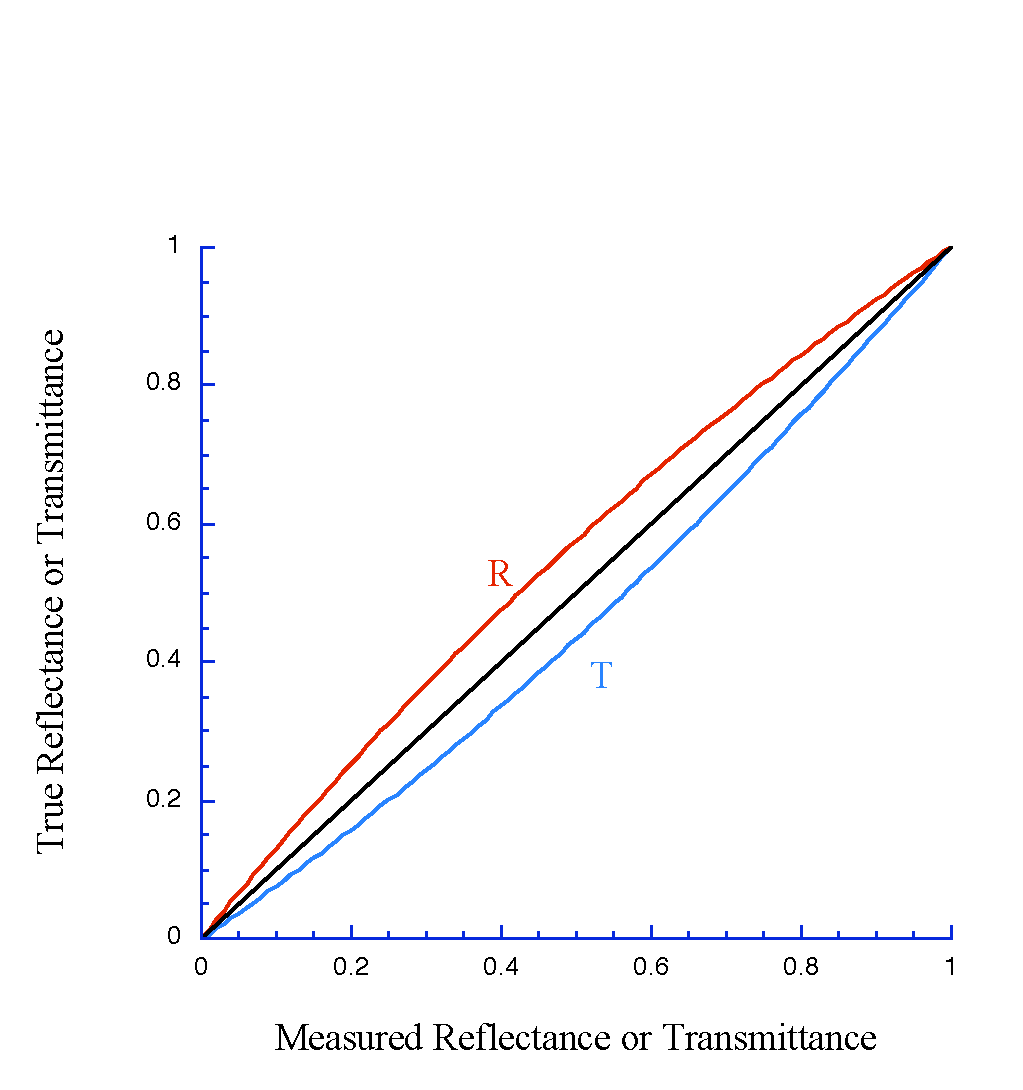
\includegraphics[width=3in]{ch3RTcorr.pdf}
\caption{The relationship between measured values using an integrating sphere
and the true values.  In this
graph, it is assumed that the dark measurement was completely dark and that
the reflectance standard was 100\%.  These effects are typical for a relatively
large sample port (50\,mm port) in a moderate size integrating sphere (200\,mm diameter).
In general the measured values using an integrating sphere will tend to underestimate reflectance measurements ($M_R<R$)
and overestimate transmittance ($M_T>T$).}
\label{spherecorr}
\end{figure}

Unfortunately integrating spheres do not
have a linear response to different sample reflectances (see Figure~\ref{spherecorr}).
This graph shows that the corrections needed for the sphere are least at
the two ends, and highest in the center.  The corrections needed for the
center depend on the geometric size of the sphere and ports as well as
on the sphere wall reflectance.  To minimize the need for these corrections,
it is best to use a reflectance standard that is slightly higher than all
the sample reflectances.  This will reduce the magnitude of the sphere 
corrections and therefore the sensitivity of your measurement to integrating
sphere parameters.

The magnitude of the sphere correction can be huge.  For example, we were making
measurements\footnote{Hi Beatriz!} on non-scattering, dark polyurethane samples
using the substitution (single-beam) method.
Now, the index of refraction of polyurethane is $\sim$1.5 and therefore the 
reflectance of the sample will be at least 4\% due to specular reflectance.
However, our measurements were consistently giving us 3\%.  The ultimate reason
was that the sphere efficiency (gain) was so much greater for the standard reflectance
measurement than it was for the sample reflectance measurement that when
calculating $M_R$ it came out 25\% lower than expected.  Obviously, this effect
would have been mitigated if we had followed my own advice and used a dark
reflectance standard, but I am sure that I had a good reason for ignoring myself.

\subsection{Which integrating sphere?}
There is a long history of the use of integrating spheres%
\cite{sumpner92,ulbricht00,taylor20,jacquez55,goebel67,pickering92}.  Good 'ole  Ulbricht
proposed the first one a hundred years ago\cite{ulbricht00}.  You can make your own easily.  Just
get a sphere, e.g., a child's ball and cut it in half.  Paint the inside with
BaSO$_4$, glue it back together attach detectors and voil\'{a}!  Or you can plunk
down a thousand bucks and buy one from LabSphere.  

The integrating sphere is characterized by its diameter, its ports, its baffle,
and its wall reflectance (typically $\sim$98\%).  In all the discussion and
code that follows, it is assumed that the baffle (inside the sphere) is located
between the sample and the detector.  This ensures that all the light leaving 
the sample hits the diffuse white coating on the sphere walls and is more-or-less
uniformly distributed across the sphere walls.  If the baffle is not present, then
some (unknown) fraction of light directly propagates from the sample to the
detector, while the rest of the light bounces around in the sphere.  It is
possible approximate the light captured by the detector and sample, but this
depends on the extent of the emission profile from the sample, the geometry
between the sample and the detector, as well as on the reflectance of the
detector at that angle.  It is much better just to require the presence of a
baffle and avoid the whole mess.  

The size of the sphere is usually determined by what sphere you happen to
have in the lab.  The sphere diameter pretty much determines the maximum
sample port size.  The theory of integrating spheres assumes that the sphere
is spherical in shape.  Obviously if you create a port in the sphere by 
slicing off a large chunk of the sphere and then place a flat sample 
on of the sample port you will no longer have a perfect sphere.  A rule of
thumb is that you do not want the sample area to be more than 10\% of the
sphere wall area.  

The size of the sphere dictates the largest sample size, but the illumination
beam determines the smallest sample size.  Ideally the entire beam would hit the
sample.  In a transmittance experiment, light that misses the sample is a
disaster because that light is difficult to properly measure experimentally.%
\footnote{One might argue that the light does not enter the sphere at all and therefore
will be properly accounted for by the calibration measurements.  This is true, but
(1) the calibration measurements will be exquisitely sensitive to shifts in the beam
profile, (2) you are throwing away some signal immediately, and (3) by illuminating
with a beam that is equal to the entrance aperture, you are maximizing losses out
the edge of the sample---these are accounted for by \iadprog{}, but will cause 
\iadprog{} to run much more slowly because multiple attempts will be needed to
properly calculate the light losses.}
Light that misses the sample in a reflectance measurement is less problematic.
That light should be properly accounted for by the calibration measurements, but
the light that misses the sample significantly adds to the background noise
in the reflectance measurement.

The sample size is also connected to the sample thickness.  Generally, one
wants to have large aspect ratios for the sample (port diameter is ten times
the sample thickness.)  So for example, a beam 1\,mm in diameter, 
a sample 1\,mm thick, a port 10\,mm in diameter, and a sphere 100\,mm in diameter 
are all reasonable, practical values.

\subsection{How many spheres?}

This seems simple right?  Why have a whole section devoted to counting the number 
of spheres?  Well, mostly because the program treats the cases of 0, 1, and 2
spheres differently.  The \iadprog{} program always reads the same number of sphere parameters at the beginning of each data file (i.e., from the header).  Therefore, even
if you specify zero spheres, you will need to include values for two spheres 
in every data file.\footnote{Insane, I know, but the original \iadprog{} did not require this,
and automated processing became tricky.  It was surprisingly
hard to maintain the code and unnecessarily confusing.  Now I figure that it is easier
for me to make you copy-and-paste sphere parameters than it is for me to continually update
\iadprog{}.}

\subsubsection{Zero}

When you specify 0 spheres, then the program assumes that 
you have made measurements of the sample in such a way that the values that you
specify for $M_R$ and $M_T$ are devoid of integrating sphere errors and therefore
\iadprog{} \textit{ makes no corrections for the integrating spheres.}  Good
reasons for choosing this are
\begin{itemize}
\item
You just want to get a quick estimate and can't be bothered to type in the
five parameters needed to characterize the sphere (even though I made it really,
really, easy for you.)
\item
You are making your measurements using the comparison method (dual beam) \textit{and}
you don't think that the uncollected light from the initial direct illumination
is significant.
\item
You want to evaluate how much an effect the sphere corrections are having on
your final derived optical properties.\footnote{There is a simpler
way to do this, just specify \texttt{-s} as a command line switch when processing
your data.}
\item
You don't know the sphere wall reflectivity.  If you want to have robust measurements
then there is some merit in determining the reflectivity as outlined in this document.
This measurement is consistent with the basic assumptions made in the program and
helps to eliminate some sorts of systematic errors.
\end{itemize}


\subsubsection{One}

When you specify 1 sphere, then a single sphere is assumed to have been used to 
measure the sample reflectance and transmittance.  This does not have to be the
same sphere, but it is assumed that a second sphere is not present in a way that
it affects the results of the sphere making the measurements.
\textit{The program will use the values in the header to make corrections
for a single sphere.}  The values for the reflection sphere and the transmission
sphere do not need to be identical --- a single sphere means that one sphere is
used at a time for all measurements. 

\subsubsection{Two}

Using two spheres is actually why I was originally interested in this problem.%
\footnote{Back in the day, laser heating and coagulation of tissue was
\textit{the} application of interest.  Since no one knew how the optical properties
changed during high power irradiation, I tried to measure the changes in optical
properties as they changed.}
There are a few good reasons to use two spheres.  First, if the
sample is has dynamically changing optical properties, then it is critical
that both $M_R$ and $M_T$ be measured at the same time.  Another reason 
might be that you would like to measure the greatest number of samples in
the shortest possible time.  

Nevertheless, there are a couple of drawbacks to using two spheres at once.
The first drawback is the prosaic problem of making good contact on both sides of
the samples with the spheres.\footnote{One of our spheres was dropped and
one port is not parallel to the port on the opposite face.  Since the internal
light baffles pretty much determine the necessary sphere orientation, this makes
double integrating sphere measurements tricky.}
One does not want to squish one side of the sample so that just barely adequate
optical contact is reached on both sides.  The second drawback is that it is
a pain in the neck to make the calibration experiments.  

\subsection{What about dual-beam spectrometers?}

Dual-beam spectrometers use two beams:  the sample is placed in one beam
and a reference is placed in the second beam.  Two measurements are made (usually
sequentially) and the reference beam is used to correct for system effects like
lamp variation with wavelength or detector changes or anything that affects the 
light path.  For example, two cuvettes might be used with one cuvette being a
reference that allows most of the effects of specular reflection from surfaces to
be corrected.
We are most interested when two beams are used in an integrating sphere.  
The two common beam geometries are shown below
\\
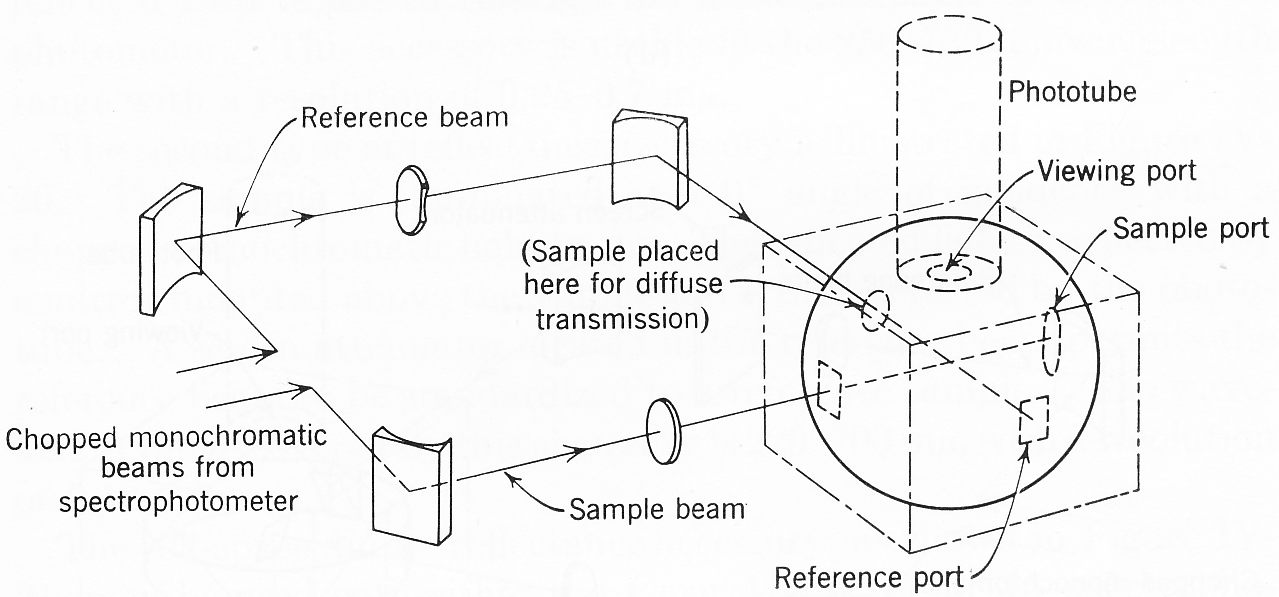
\includegraphics[width=2.3in]{dual90.png}
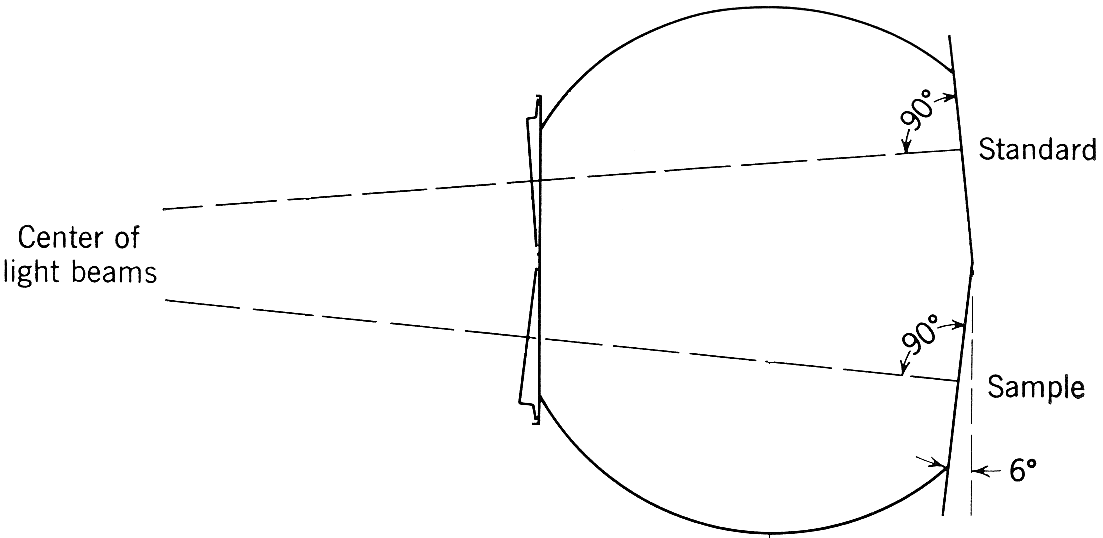
\includegraphics[width=2.3in]{dual8.png}\\
in these two (modified) images~\cite{wendlandt66}.  In both these examples
the beam is incident perpendicular to the samples, but the angle between
the beams might be ninety degrees (left) or shallow (twelve degrees on the right).

So why do I, or actually you, care?  The geometry implies a different method
of normalization.  The good part is that ``sphere corrections'' are not needed
any longer.  Because both the reference and the sample are present in the sphere
during reference and sample measurements, the sphere efficiency remains constant
and no ``sphere corrections are needed.''  

Light losses are another issue.  The direct light loss is completely unaccounted
for in the dual-beam sphere.  Oddly, the diffuse light loss \textit{is} properly
accounted for because the diffuse sample reflectance only enters into the calculation
when figuring out the integrating sphere efficiency.  Since the sphere efficiency
for the sample illumination and the standard illumination are equal, the diffuse
light loss is not an issue.

Anyhow, if you are using a dual beam system, then if your system automatically
gives you the ratio of the sample reflectance to the standard reflectance, you
will want to calculate $M_R$ 
$$
M_R = r_{\mathit{std}} (R_s - R_0)
$$
where $R_0$ is a measurement obtained with nothing in the sample reflection port and is present
to correct for light that misses the sample and hits the
sphere wall first.  The value for  $M_T$ is similar
$$
M_T = t_{\mathit{std}} (T_s - T_0)
$$
although now $T_0$ is made with a blocked sample port and represents the least amount
of light that may be measured.

How does one analyze these in practice with IAD?  Well, the simplest way is to just
to use the \texttt{-X} option\footnote{The `X' is for crossed beams.} and specify
the sphere parameters that you used.

\subsection{How should the sample be prepared?}

There are a whole host of experimental problems which plague measurements
of reflectance and transmittance.  Inattention to experimental details will yield
garbage.  Just look at the variation in the optical properties
gathered together in Cheong \emph{et al.} \cite{cheong90a}.  These can be attributed
to two sources of error---inattention to the details of the experimental
measurement and to flaky optical models.  Since presumably, the adding-doubling
method is \textit{not} flaky, you are saved from the second source of error.  
But I can do nothing about saving you from poor experimental technique
except to warn you about various things.  

\subsubsection{Freshness}
If the sample is not fresh then optical properties will differ from those
measured {\it in vivo}.  Obviously, the tissue begins rotting as soon as
its nutrient supply is removed. If the tissue is not in excellent condition then
there will be problems.  By the way, there has been essentially no work
done on the changes in optical properties which take place when a tissue
is removed.  There has been minor work done on the changes in optical
properties with heating, but nothing to that definitively says that the
optical properties measured \textit{ex vivo} are even close to those 
\textit{in vitro}.  

\subsubsection{Boundaries}
The need for glass or quartz slides at the boundaries is caused by
the rough surface of most tissues.  Since the boundaries are characterized
by Fresnel reflection, it is relatively important for the experiment to
match the quantities calculated by the code.  Water, saline, or best
phosphate buffered saline (PBS) or some
other fluid should be used to ensure good index matching between
the tissue and the slide.  Care should be taken to ensure that no bubbles 
are formed between
the slide and the tissue.   Since the index of refraction
of glass is 1.5 and that of tissue ranges from 1.33 to say 1.45, the 
boundaries are not perfectly matched.  You just have to live with this
or experiment with various immersion oils and various glasses and plastics
achieve perfection.  

\subsubsection{Hydration} 
Optical properties of the sample definitely change with the amount of water in the
tissue.  It is important to store the tissue in air-tight containers
sandwiched between moist (with PBS) towels at cool (above
freezing) temperatures.  If you don't believe me, then leave a piece of
tissue exposed to air for 48 hours.  It will appear quite different from
fresh tissue.\footnote{Your co-workers will probably complain
bitterly about the smell, but we are only concerned about the appearance of
the tissue.}  Since your eye sees reflected and transmitted light, any
measurements will also differ.

\subsubsection{Sample Diameter}
How big should the sample be?  First, it must be larger than the sample port
in the integrating sphere.  If not, then make the port smaller.  Second,
you want the distance from the edge of the irradiating beam on the sample
to the edge of the port ($h$) to be as large as practicable. If,
\begin{eqnarray*}
h \gg {1\over \mu_a+\mu_s'}
\end{eqnarray*}
then relatively little light will be lost out the sides of the sample.  
``Relatively little'' is a complex and depends on other things.  In general,
it is hard to predict without modelling carefully.  Before the Monte Carlo
correction was added to this code, all losses would be attributed to absorption.  Consequently, any absorption coefficients generated for this sample will be too large.  The ramifications now are less dire: lost light takes longer to analyze because
the amount of lost light must be continually recalculated.  

\subsubsection{Variability}
 From spot to spot on one sample and from sample to sample.  Make enough
measurements that you have some idea of the average value and variance for
each sample as well as the variability from sample to sample.

\subsubsection{Blood} 
Should samples be measured with or without blood?
Clearly neither really is a good example of the in vivo situation.  If
samples have no blood then the optical properties of the sample itself are
being measured.  The contribution to blood can be added later.

\subsubsection{Freezing}  
To obtain very thin subsections it is necessary to freeze the sample.  Rumor
has it that the freezing process changes the optical properties.  The
evidence for this has been on muscle tissue.  Other tissues like aorta and
dermis are different and not so susceptible to freezing artifact.

\subsubsection{Interference}  
Serious pain in the wahzoo.  The interference usually comes from multiple
internal reflections from the glass
slides which sandwich the tissue sample.  When a laser beam strikes the
air-glass surface it is reflected.  It is also reflected at the
glass-tissue surface.  This reflectance can interfere with the first
reflectance. One would expect this to be a neglible effect, but in practice
it can nearly 10\%.  It is easily demonstated by placing a microscope
slide in the path of a laser beam and measuring the transmission.  Then
move the slide slightly and observe the transmission again.  An even more
dramatic effect is achieved when specular reflectance is measured.

What can be done?  Sit down with a box of microscope slides and go through
them one by one observing the reflectance profiles on a wall.  Discard all
those that show definite interference effects.  These should be the least
optically flat of the whole box.

Another possibility is to use very thick glass plates.  By slightly
rotating the plate the reflectance from the second surface will be
displaced sufficiently that the two beams will no longer be aligned and
consequenly will not interfere. Thick plates are not ideal because they
displace the integrating spheres and consequently all some diffuse light to
be lost before it can enter the integrating sphere.

A final posibility is to use optically flat plates.  Interference will be
constant over the surface and can be measured and accounted for.  This is
the best option, but also the most expensive.

\clearpage
\section{Measurements}

\subsection{Integrating sphere calibration}
\label{rwmeasurement}
The sphere wall reflectance $r_w$ is critical.  Hopefully, you have a new,
well-maintained sphere whose manufacturer-specified value for $r_w$ is 
accurate.  Measuring the wall reflectance $r_w$ is challenging, but can be done.  Two measurements are 
needed (figure~\ref{sphererw}),
\begin{equation}
{1\over r_w} =  a_w + a_d r_d (1-a_e) + a_s 
r_{\mathit{std}} (1-a_e) {{R^{\mathit{diffuse}}_{\mathit{std}}} \over R^{\mathit{diffuse}}_{\mathit{std}} - {R^{\mathit{diffuse}}_\mathit{0}}}.
\end{equation}
This equation illustrates the difficulty in making accurate measurements 
of the sphere wall reflectance.  The two diffuse reflectances 
$R^{\mathit{diffuse}}_{\mathit{std}}$ and $R^{\mathit{diffuse}}_\mathit{0}$ 
will only differ by the amount of diffuse light leaking from the sphere 
when the port is empty.  Consequently the difference will be small and 
any errors in the measurements will be magnified when the division is done.

\begin{figure}[!h]
\centering
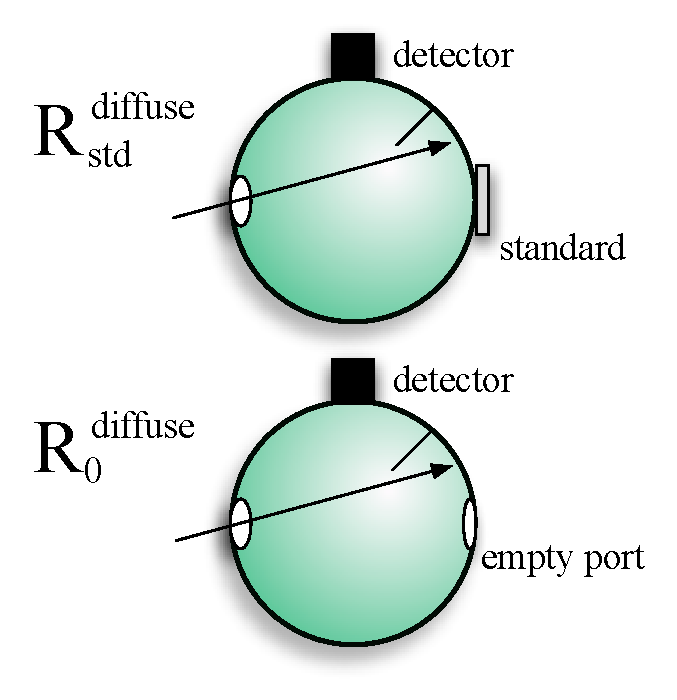
\includegraphics[width=2in]{ch3spheremeas.pdf}
\caption{The two experiments needed to determine the sphere wall reflectance.
The reason that this is a hard experiment to do well is that the quantity of
interest is the difference between the two measurements.  This is a small 
difference and is roughly proportional to the relative area of the sample
port $a_s$.}
\label{sphererw}
\end{figure}

\clearpage
\subsection{Single Sphere $M_R$ and $M_T$}

Standard usage is that \textit{reflection} is the light being reflected by the sample,
while the \textit{reflectance} is the light being reflected by the sample normalized by
the incoming light.  Reflectance has no units.  A stable useful estimate for the 
reflectance of the sample is the 
\textit{measured total reflectance} $M_R$ which is defined in terms of easily measurable
sample, standard, and background reflection measurements:
\begin{equation}
M_R \equiv r_\mathit{std}\cdot{{R(\rdirect, \rdiffuse) - R(0, 0)\over 
                    R(r_{\mathit{std}}, r_{\mathit{std}})- R(0, 0)} }.
\label{eqmr}
\end{equation}
where $R(\rdirect, \rdiffuse)$, $R(0, 0)$, and 
$R(r_\mathit{std}, r_\mathit{std})$ are defined in Figure~\ref{spherert}.%
\footnote{The value of $M_R$ differs from the true reflectance because the gain
of the integrating sphere varies with the sample reflectance (see Figure~\ref{spherecorr}).}


\begin{figure}[!b]
\centering
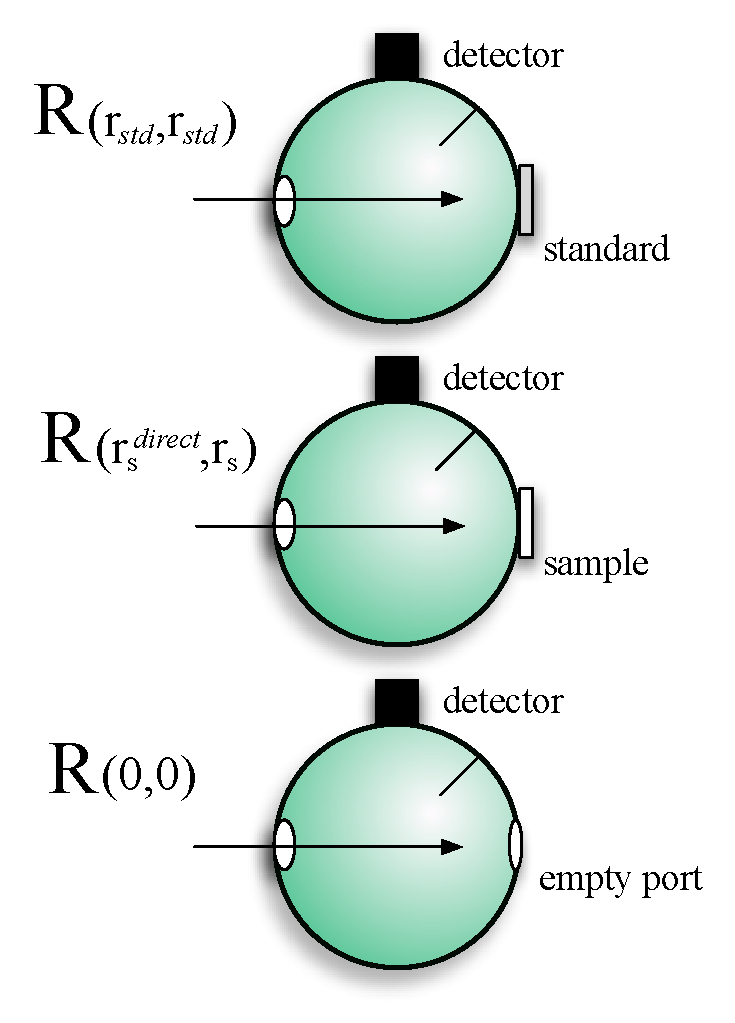
\includegraphics[width=49mm]{ch3spheresR.pdf}
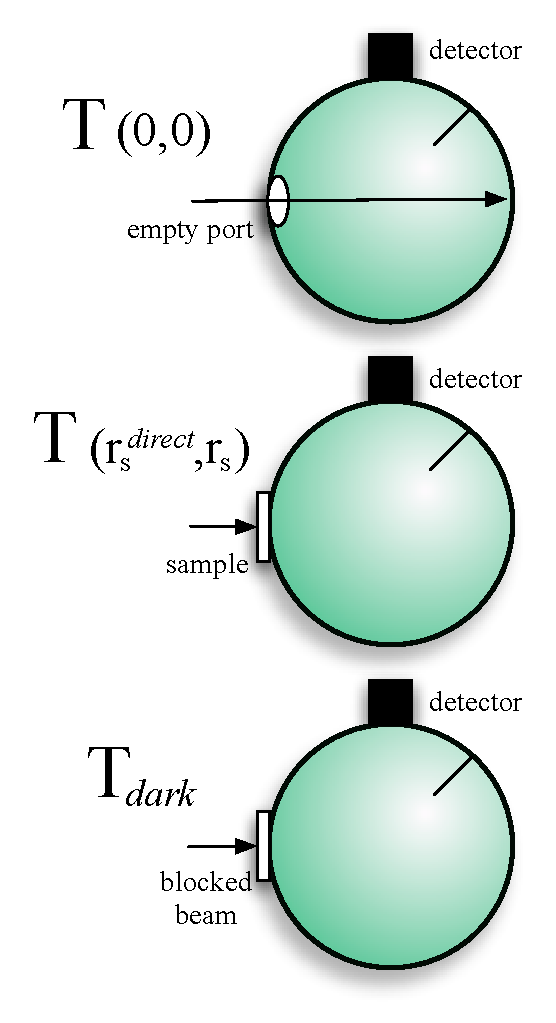
\includegraphics[width=38mm]{ch3spheresT.pdf}
\caption{The measurements needed to measure $M_R$ and $M_T$ in equations \ref{eqmr} and~\ref{eqmt}.
Note that the baffle is always located between the sample and
the detector.  The back wall of the transmission sphere is never open
(light that does not interact with the sample bounces around in the sphere).  Finally,
notice that $T_\mathit{dark}$ and $T(0,0)$ are very different.}
\label{spherert}
\end{figure}

The same idea applies to \textit{transmission} and \textit{transmittance}; the transmission
has units while the transmittance is normalized to the incident power.  The \textit{measured
total transmittance}  $M_T$ is defined as
\begin{equation}
M_T \equiv {{T(\tdirect, \rdiffuse) - T_{\mathit{dark}}\over 
                    T(0, 0) - T_{\mathit{dark}}} }
\label{eqmt}
\end{equation}
where $T(\tdirect, \rdiffuse)$, $T(0, 0)$, 
and $T_{\mathit{dark}}$ are defined in Figure~\ref{spherert}. 

\subsection{Double Sphere $M_R$ and $M_T$}

Double sphere values for $M_R$ and $M_T$ differ slightly from that for single spheres.  The experimental arrangement for the spheres in double-sphere measurements is shown in Figure~\ref{doublesphere}.  The normalized reflectance is then 
\begin{equation}
M_R = r_{\mathit{std}}\cdot{\frac{R_2(\rdirect, \rdiffuse, \tdirect, \tdiffuse)-R_2(0,0, 0,0)}{R_2(r_{\mathit{std}}, r_{\mathit{std}}, 0, 0)-R_2(0,0, 0,0)}}
\end{equation}
and transmittance by
\begin{equation}
M_T = {\frac{T_2(\rdirect, \rdiffuse, \tdirect, \tdiffuse)-T_2(0,0, 0,0) }{T_2(0, 0, 1, 1)-T_2(0,0, 0,0)}}.
\end{equation}

\begin{figure}[!b]
\begin{center}                                                            
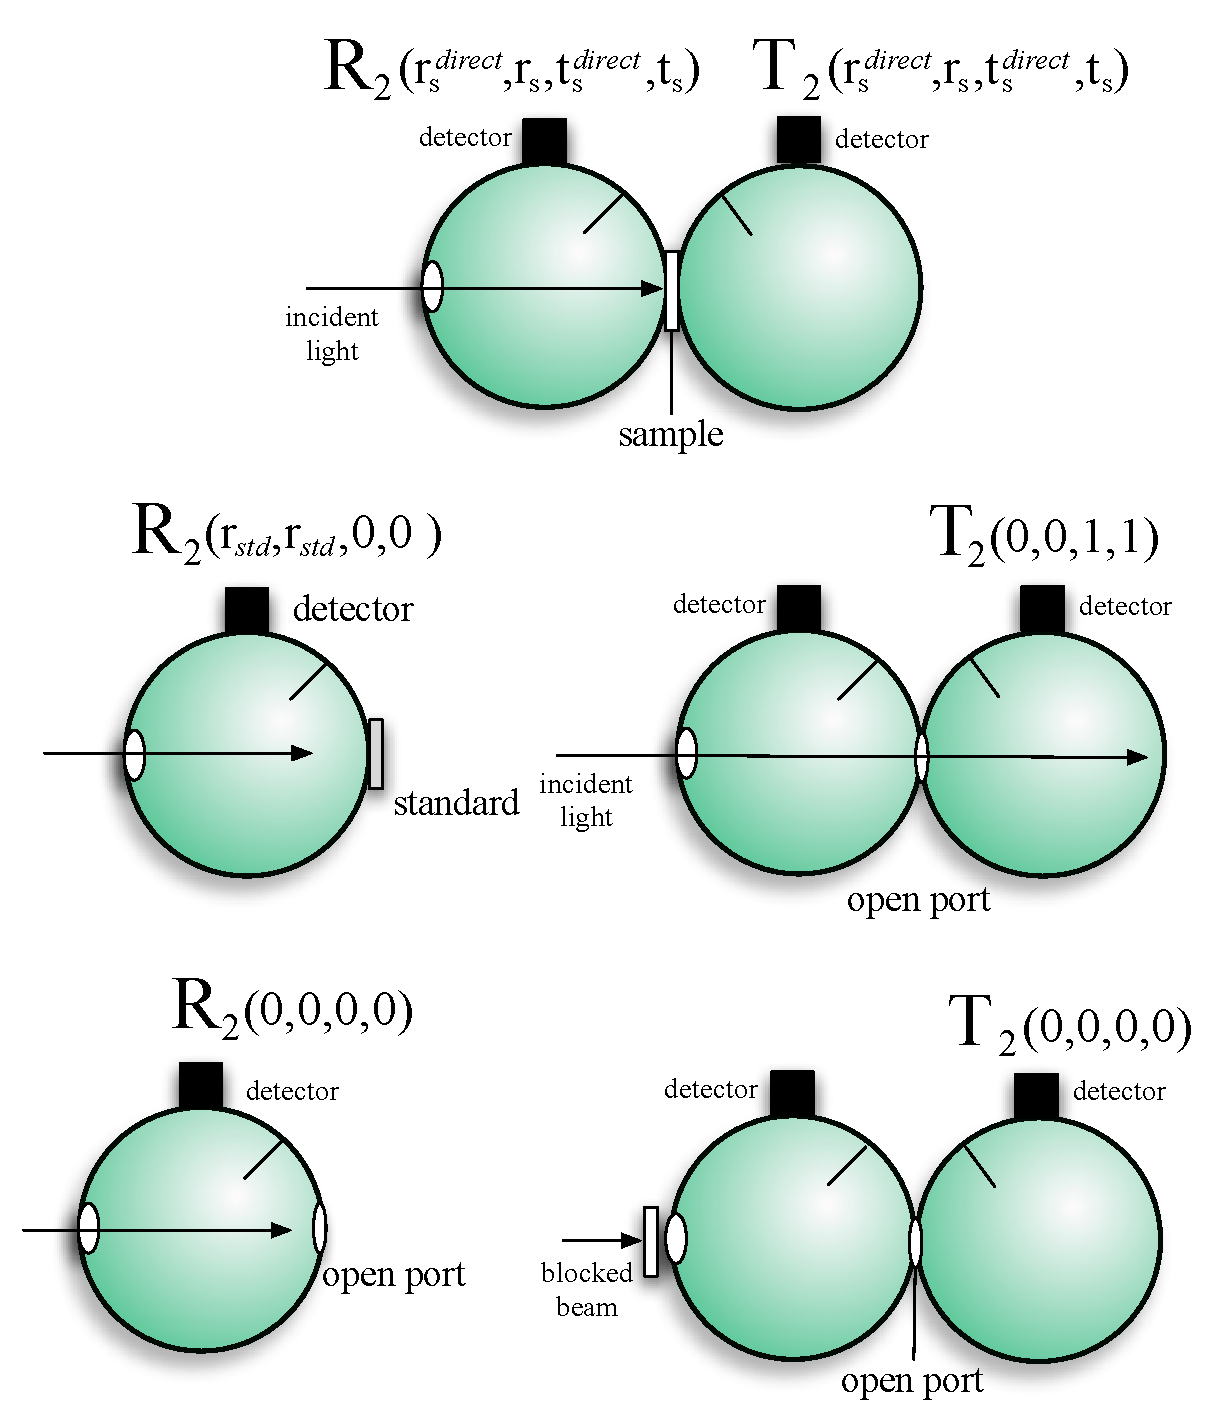
\includegraphics[scale=0.45]{ch3Doublespheres.pdf}
\caption{Measurements needed for $M_R$ and $M_T$ when two integrating spheres are used
simultaneously.}
\label{doublesphere}
\end{center}
\end{figure}

\subsection{Measured Unscattered Transmittance}

Finally, the \textit{measured unscattered transmittance} $M_U$ is the amount of light
that gets through the sample without being scattered or absorbed.
This
has been called by a bunch of different terms: collimated transmittance,
ballistic transmittance, on-axis transmittance, coherent transmittance.
\begin{equation}
M_U \equiv {U_s - U_0    \over 
            U_{100} - U_0 }
\label{eqmu}
\end{equation}
where $U$ indicated an unscattered measurement.  
In this equation, $U_s$ refers to the unscattered sample transmission,
$U_0$ is the background measurement for the unscattered transmission measurement
(beam blocked) and $U_{100}$ is the unscattered transmission measurement 
when no sample is present.

\begin{figure}[h!]
\begin{center}
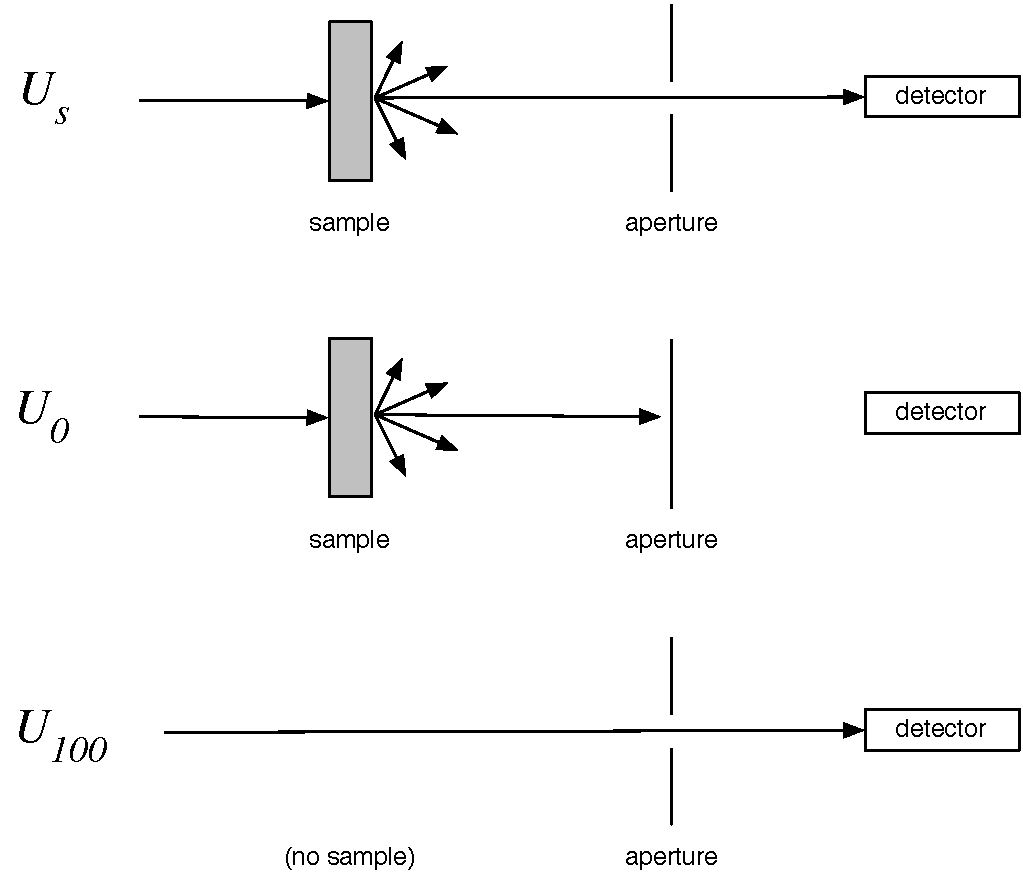
\includegraphics[scale=0.5]{colltrans.pdf}
\end{center}
\caption{Measurements needed to determine $M_U$.  }
\label{figeqmu}
\end{figure}

The measured unscattered transmittance is the most difficult measurement to make and
it is frequently underestimated how hard it is to get correct.  Be careful.  Do yourself a favor
and plot your measured values for unscattered transmittance versus
the concentration or sample thickness.  If this line is not exponentially decreasing
then you have problems.  Furthermore, you should check to make sure
that your data passes through the correct value when concentration or
sample thickness is zero.  This is easily calculated using the 
indicies of refraction.  For example, for water $(n=1.33)$ between glass slides
$(n=1.50)$ the transmittance should be roughly
$$
M_U = (0.96)(0.996)(0.996)(0.96)=0.914
$$
where I have neglected to include multiple internal reflectances.  The \iadprog{}
program does, but then it is good at that sort of thing.

Next, do a quick calculation to ensure that the amount of 
\textit{scattered light} reaching the detector is significantly less than
the estimated value for the unscattered transmittance.  Since
$$
M_U \propto e^{-(\mu_a+\mu_s) \delta}
$$ 
the value for $M_U$ gets small, very quickly!  Do
not underestimate the enormity of the smallness of $M_U$!
Remember, if your collimated transmittance data does not pass the 
above test, then the output from the \iadprog{} program must be suspect.
\emph{Garbage in, garbage out}.  It is undoubtedly better to assume
a value for the anisotropy than to use a flawed value for the
unscattered transmittance.

For scattering samples, measurement of unscattered transmittance is more
complicated because any transmission measurement 
consists of contributions from both unscattered and
scattered light.
$$
U_{\mathit{measured}} = U_{\mathit{scattered}} + U_s
$$
I can think of at least three methods for finessing this problem.%
\footnote{Aside from using optical coherence tomography (OCT) or
time-of-flight measurements}
Reasonably accurate values for the measured unscattered transmittance
can be obtained by make measurements at (1) various distances, (2) various
angles, (3) with very thin samples in
which the contribution from scattering is negligible.  The last two
methods are described in the paper by Jacques, Alter, and Prahl~\cite{jacques87b}.
The other method has not been
published (as far as I know---since I thought it up and have not had the
time to go to all the trouble to write it up and review the literature.)%
\footnote{I should probably mention that polarization can also be used to increase
the collimated to scattered ratio.  Unfortunately this only attenuates the
diffuse contribution by a factor of two for thick samples (whose diffuse
transmittance will be unpolarized.)}

If the light incident is perfectly collimated (no divergence) and the
scattered light is isotropically distributed over all angles,%
\footnote{This is a surprisingly good approximation when
more than two scattering events take place in the sample.} then the
amount of light dectected at a distance $z$ from the sample is
\def\sa{\begin{array}{c}}
\def\ea{\end{array} }
$$
\sa\mbox{Measured}   \\ \mbox{Power}      \\ \mbox{[W]}           \ea =
\sa\mbox{Scattered}  \\ \mbox{Intensity}  \\ \mbox{[W sr$^{-1}$]} \ea \times
\sa\mbox{Detector}   \\ \mbox{Solid Angle}\\ \mbox{[sr]}          \ea +
\sa\mbox{Collimated} \\ \mbox{Irradiance} \\ \mbox{[W cm $^{-2}$]}\ea \times
\sa\mbox{Detector}   \\ \mbox{Area}\\ \mbox{[cm$^2$]}      \ea
$$
where the
solid angle subtended by the detector located at a distance $z$ from the
sample is
$$
\mbox{detector solid angle}=
	{\mbox{area of detector}\over\mbox{area of sphere with radius $z$}}
$$

If the scattered light exiting from the back of the sample is isotropic
then the intensity  for this light will have a constant value $I_\mathit{scat}$.  
Therefore, if the irradiance is $E_0$ then the unscattered transmission
measurement will be 
$$
U_{\mathit{measured}}=
	{I_{\mathit{scattered}}\over 4\pi z^2 } + U_s
$$
Notice that the first term (the scattered light) decreases with the sample
detector separation $z$. For a perfectly collimated beam $U_s$ will be
independent of the distance $z$, and therefore
the first scattered term may be made as small as desired by moving the sample
farther and farther from the sample. 
$U_s$ is the limit of as the separation between sample and
detector becomes infinite.   Thus, if $U_{\mathit{measured}}$ is known for
several distances between sample and detector, linear regression might
yield both $U_s$ and the scattered intensity.%
\footnote{
A major assumption in this development is that the scattered light
exiting the sample is isotropic.  This is true for optically thick samples
but definitely not for  optically thin ones \cite{jacques87b}.}

\clearpage
\section{The Data File}

The basic structure of the data file consists of a header section followed by your
measurements of reflectance and transmittance.  The header describes
details of the experiment: the sample thickness, the beam diameter, the
indices of refraction, the number and geometry of the spheres used.%
\footnote{Details about \textit{how the measurements should be
analyzed} are handled by command-line options (next section).
This allows one (for example) to assume different default anisotropies, a different
number of quadrature points, or different constraints on the Monte Carlo
simulations.  Of course, this is also a lie.  I have extended the number
of command-line parameters to allow one to specify all the parameters in
the header of the data file.  This allows one to do an IAD calculation
without needing to create an input data file, which I find to be useful
when scripting tasks --- or asking \textit{what if} questions from the
command-line.} 


\subsection{The header}
The header was designed to be
\begin{enumerate}
\setlength{\itemsep}{0pt}
\item easily annotated for humans
\item sufficiently flexible to accommodate all common experiments
\item readily parsed by machine
\item filled with entries that have a simple physical meaning
\item a complete description of experimental geometry
\item devoid of rarely-used parameters
\end{enumerate}
These goals were achieved by carefully specifying a minimal set of
parameters that describe a particular experiment and developing a
simple comment style.  At its simplest, the header consists of the
identifying tag \texttt{IAD1} followed by eighteen numbers.

The first four characters of the file must be \texttt{IAD1}.  
This allows the program to do basic sanity checking of the file before 
beginning to parse the file.  The final digit may one day be used as
a version number.  I hope not.  Anyway, one example of a valid
header is the sequence
\texttt{IAD1} followed by 18 numbers,
\begin{center}
\begin{minipage}{8cm}
\scriptsize
\begin{verbatim}
IAD1 1.34 1.5 1 1 5 .96 1 203.2 25.4 12.7 1 .96 203.2 25.4 12.7 1 .96 2 
\end{verbatim}
\end{minipage}
\end{center}
This short example is functionally identical to the longer annotated example
that is shown below.  Of course, this version is not suitable for human consumption.  
Nevertheless, it demonstrates that (1) the comments help readability tremendously, (2) the quantity of the parameters is fixed, and (3) the ordering is fixed.

To make my life easier, I allow and nearly always use comments.
A number sign (\#), aka octothorpe, pounds sign, or hash symbol is used to start a comment; everything
from the number sign to the end of the line will be ignored.
White space and comments are ignored except when following a number.  There
is no difference between comments, tabs, spaces, linefeeds, or carriage returns; any
one will end a number. 

\begin{center}
\begin{minipage}{8cm}
\scriptsize
\begin{verbatim}
IAD1   # Must be first four characters

# Input Example with a single set of sphere coefficients
# The order of entries is important 
# Anything after a '#' is ignored, blank lines are also ignored
 
1.34   # Index of refraction of the sample
1.50   # Index of refraction of the top and bottom slides
1.0    # [mm] Thickness of sample
1.0    # [mm] Thickness of slides
5.0    # [mm] Diameter of illumination beam
0.96   # Reflectance of the calibration standard

1      # Number of spheres used during each measurement

       # Properties of sphere used for reflectance measurements
203.2  # [mm] Sphere Diameter  (8 in * 25.4 mm/in)
25.4   # [mm] Sample Port Diameter
12.7   # [mm] Entrance Port Diameter
1.00   # [mm] Detector Port Diameter
0.96   # Reflectance of the sphere wall

       # Properties of sphere used for transmittance measurements
203.2  # [mm] Sphere Diameter  (8 in * 25.4 mm/in)
25.4   # [mm] Sample Port Diameter
0.00   # [mm] Entrance Port Diameter
1.00   # [mm] Detector Port Diameter
0.96   # Reflectance of the sphere wall

2      # Number of measurements, M_R, M_T
\end{verbatim}
\end{minipage}
\end{center}
In this annotated header, the details of the
geometry of the experiment are immediately apparent: reflectance
and transmittance was measured using a single sphere in which 
the 12.7\,mm diameter sample was illuminated by a 5\,mm diameter beam.
We also know that the sample was sandwiched between glass slides
($n=1.5$) that were 1\,mm thick.

The last number in the header determines how many measurements are available.  This number may vary from 1 to 6 depending on the experimental circumstances.  

When using one reflectance sphere, the entrance port diameter defined as the size of the
port though which light enters the sphere.  The sample port is the size of the hole
in the sphere that is adjacent to the sample.\footnote[1]{The actual sample size is
always assumed to be larger than the sample port.  In fact, the sample is assumed
to have infinite lateral extent.  It is a challenge when working with small pieces
of tissue to maintain a large port size and still have the sample port completely
covered by the sample.}  Finally, the detector port diameter
is the size of the port that houses the detector or optical fiber that goes to the
detector.  The reflectivity of all the ports is assumed to be zero --- i.e., the 
ports are black.

If your detector is not round, but rectangular, then the detector diameter should 
be chosen to match the area of your detector.  Thus if your detector is a rectangle
10$\times$1\,mm$^2$, you would use a diameter of $\sqrt{40/\pi}\approx3.6$\,mm.
Furthermore, if you have multiple detectors in your sphere (e.g., for different wavelength
regions), the detector diameter should correspond to area equal to the sum of all
the detector areas.  

When using one transmission sphere, the entrance port should be set to zero.  We are
assuming direct collimated illumination of the sample.  The sample port size should
be set to the size of the port next to the sample.  The detector size should be set
as described above.  The reflectance and transmittance spheres differ in the number
of places that light can be lost.  A reflectance sphere loses light out the entrance
port, the detector port, and the sample port (through the sample).  A transmittance
sphere loses light only from through the detector ports and the sample port.\footnote[1]{Of
course, in our current set up in the lab, we have mounted the reflectance fiber 
permanently in one sphere that is used for both transmittance and reflectance
measurements.  In this case, there are identical causes of light loss in both
spheres and therefore the entrance port size in the transmittance sphere might
be non-zero or this area could be lumped into the detector port size.  In practice
it is just easiest to make the parameters for both spheres be equal to one another.}


\subsection{The data section}

After the header comes measurements of the reflectance $M_R$ and transmittance $M_T$.  
This is sort of a wonky section because I wanted to have a reasonable amount of flexibility;
this especially handy when combined with unix scripting to automatically process large numbers 
of integrating sphere measurement files.  The organization is not \textit{that} confusing, but 
you should read this section to understand why things are the way they are.  My rationale will 
not make the layout any less kludgy, but it may provide a modicum of
amusement where otherwise there would only be anger and frustration.

Ideally one
would always have three (or more) measurements.  Unfortunately, often the unscattered
transmittance measurement is not available.  For example the the amount of unscattered
light that propagates through a millimeter of tissue is very small.  For thicker samples
the total transmitted light 
$M_T$ is zero also. In this case then only one parameter can be measured.  The following
describes how you deal with multiple columns of data.

\subsubsection{White space}

The same rules for white space and comments that apply in the header section
also apply to the data section.  This means that you can liberally comment your
data (or not) by using \texttt{\#} to start a comment.

\subsubsection{Optional wavelength entry}

The \iadprog{} program is mainly intended to analyze spectral measurements of reflectance
and transmittance.  For a number of reasons (e.g., graphing) it is convenient to 
precede the measured values by the appropriate wavelength,
\begin{center}
\begin{minipage}{4cm}
\scriptsize
\begin{verbatim}
#lambda	   M_R      M_T
 800     0.16830  0.24974
 810     0.16271  0.26479
 820     0.16289  0.25530
\end{verbatim}
\end{minipage}
\end{center}
Since we don't want to require wavelength data, it would be nice if \iadprog{} should also give identical results for input data like this
\begin{center}
\begin{minipage}{3.5cm}
\scriptsize
\begin{verbatim}
#  M_R      M_T
0.16830  0.24974
0.16271  0.26479
0.16289  0.25530
\end{verbatim}
\end{minipage}
\end{center}
There are at least two possible solutions to solve this problem: add another parameter to the header or auto-recognize
the presence of a wavelength.  Since I wanted to keep the number of parameters in the
header to a minimum, I went with the second option.  This leads to the following rule.

\textit{If the first
number on a line is greater than one, that number is assumed to be a wavelength, 
otherwise it is interpreted as $M_R$.}  

The value of the wavelength is not used anywhere
except for being copied to the output file.
The above rule means that you cannot measure your wavelength in microns if that forces
the wavelength to fall between 0 and 1.  For example 532.8 is fine as a wavelength
but 0.5328 will be interpreted as a value for $M_R$.  This is why all the example
files in the test directory use nanometers for the wavelength range.

\subsubsection{One measurement}

\begin{center}
\begin{minipage}{3cm}
\scriptsize
\begin{verbatim}
#lambda	   M_R  
 800     0.16830
 810     0.16271
 820     0.16289
\end{verbatim}
\end{minipage}
\end{center}

When the only measurement specified, it is assumed to be the measured reflectance $M_R$.
Since there is only a single measurement two assumptions are made:
\begin{itemize}
\item
the optical thickness of the slab is assumed infinite and 
\item 
the anisotropy
coefficient set to the default value ($g=0$ unless a specific command-line 
value has been specified).  
\end{itemize}
The albedo is varied until the correct value
for the measured reflectance $M_R$ is obtained.  Now \iadprog{} generates both absorption
and scattering coefficients.  Because only the albedo is known,
and \iadprog{} reports both the scattering and absorption, some value for the
scattering coefficient is assumed ($\mu_s=1$).  There is really no good reason for this
other than the general observation that scattering is relatively constant
(as a function of wavelength) for most samples that are measured.  One might 
process a reflectance-only data set to get a 
sense of how absorption varied across the range of input values.

More recently, I have expanded the command-line options for \iadprog{}.  This
means that if you happen to know the absorption coefficient and have a reflectance
measurement you might try
\begin{verbatim}
prompt> iad -A 0.01 -g 0.6 file.rxt
\end{verbatim}
which will constrain the $\mu_a=0.01$\,mm$^{-1}$ and the $g=0.6$.  Therefore
the scattering coefficient will be found.

\subsubsection{Two measurements}

\begin{center}
\begin{minipage}{6cm}
\scriptsize
\begin{verbatim}
#lambda	   M_R      M_T
 800     0.16830  0.24974
 810     0.16271  0.00000  #treated as one measurement
 820     0.16289  0.25530
\end{verbatim}
\end{minipage}
\end{center}
This is the most common case and
\begin{itemize}
\item 
the anisotropy
coefficient set to the default value ($g=0$ unless a specific command-line 
value has been specified).  
\end{itemize}
The first two values are the measured
reflectance and the measured transmittance. As long as
$M_T \ne 0$ then the anisotropy coefficient set to the default value and
the albedo and optical depth are varied until the correct values of $M_R$ and 
$M_T$ are obtained.  The scattering and absorption coefficients are calculated
from the final values for the albedo and optical depth and printed. When $M_T=0$
then the situation is identical to the one measurement case above and is treated
in exactly the same way.

\subsubsection{Three or more measurements}

\begin{center}
\begin{minipage}{8cm}
\scriptsize
\begin{verbatim}
#lambda	   M_R      M_T      M_U
 800     0.16830  0.24974  0.0012
 810     0.16271  0.00000  0.0000 #treated as one measurement
 820     0.16289  0.25530  0.0000 #treated as two measurements
\end{verbatim}
\end{minipage}
\end{center}
If both $M_T\ne0$ and $M_U\ne0$, then $M_U$ is used to calculate
the optical thickness directly.  The optical thickness is calculated by including
all the multiple internal reflections in the slide and sample and
using $M_U$.  
The albedo and anisotropy are varied until $M_R$ and $M_T$ are
matched. 

If $M_U=0$ but $M_T\ne0$, then the situation is identical to the two measurement
case above.  Finally when both $M_T=0$ and $M_U=0$ then the single measurement 
case above applies.

\subsubsection{Four measurements}

\begin{center}
\begin{minipage}{8cm}
\scriptsize
\begin{verbatim}
#lambda	   M_R      M_T      M_U     r_w
 800     0.16830  0.24974  0.0012   0.951
 810     0.16271  0.00000  0.0000   0.952 #treated as one measurement
 820     0.16289  0.25530  0.0000   0.953 #treated as two measurements
\end{verbatim}
\end{minipage}
\end{center}
This is how \iadprog{} handles the situation in which the sphere wall reflectance varies
with each measurement (e.g., as a function of wavelength).  Both the
reflectance sphere and the transmittance sphere wall reflectances are
changed by this value.  If you want to use this option when you only
have one or two measurements, then indicate that you have four measurements
and enter 0.00 for the unknown values (as in the 810\,nm line above).
This option was originally needed because we needed to use a sphere that was coated
for use in the visible with wavelengths from 1,000--1,600\,nm.  In this region the wall reflectance
changed significantly over the wavelength range that we were using.

The real advantage of including the sphere wall reflectance measurements $r_w$
that were made according to section~\ref{rwmeasurement} are that it negates a
variety of systematic errors that might be present in your measurement.  Since
the $r_w$ measurement is made with the same light source, detector, spheres, and
standards \textit{and} is analyzed using the same set of integrating sphere 
assumptions as the $M_R$ and $M_T$ measurements, the two sets of measurements
are consistent.  To put it bluntly, if LabSphere says your sphere has a reflectance
of 0.995 and you measure a value of 0.980, I would assert that your value is
more appropriate for analyzing your integrating sphere measurements.  

\subsubsection{Five measurements}

\begin{center}
\begin{minipage}{8cm}
\scriptsize
\begin{verbatim}
#lambda	   M_R      M_T      M_U     r_w    t_w
 800     0.16830  0.24974  0.0012   0.951   0.980
 810     0.16271  0.00000  0.0000   0.952   0.981 #treated as one measurement
 820     0.16289  0.25530  0.0000   0.953   0.982 #treated as two measurements
\end{verbatim}
\end{minipage}
\end{center}
This is how \iadprog{} handles the case of spheres with
different reflectances as a function of wavelength.  Typically if the
wall re is changing, then so will the sphere wall reflectance.  Of course,
if the wall reflectance is not changing then just fill in the same value
each time.  Like the four measurement case, if $M_U$ or $M_T$ is unknown,
then just enter zero.

\subsubsection{Six measurements}
The insanity continues and we allow the reflectance
standard to have some spectral character.
\begin{center}
\begin{minipage}{8cm}
\scriptsize
\begin{verbatim}
# nm    M_R    M_T    M_U    r_w   t_w    rstd
 550  0.0731 0.9307 0.0000 0.9788 0.9788 0.9800
\end{verbatim}
\end{minipage}
\end{center}
Typically if the wall reflectance is changing, then so will the 
standard reflectance.  Of course,
if the wall reflectance is not changing then just fill in the same value
each time.  Like the five measurement case, if $M_U$ or $M_T$ is unknown,
then just enter zeros.

\subsubsection{Seven measurements!}
The insanity finally ends.  The default transmittance for
100\% transmission gets specified also.
\begin{center}
\begin{minipage}{8cm}
\scriptsize
\begin{verbatim}
# nm    M_R    M_T    M_U    r_w   t_w    rstd   tstd
 550  0.0731 0.9307 0.0000 0.9788 0.9788 0.9800 1.0000
\end{verbatim}
\end{minipage}
\end{center}

\subsubsection{Putting it all together}
\begin{table}
\begin{center}
\begin{minipage}{8cm}
\small
\begin{verbatim}
IAD1
#
# Tests using calculated values for M_R and M_T
# by Scott Prahl
#
1.4          # Index of refraction of sample
1.0          # Index of refraction of top slide
1.0          # [mm] Thickness of sample
1.0          # [mm] Thickness of slides
2.0          # [mm] Diameter of illumination beam
1.00         # Reflectance of calibration standard

0            # [mm] Number of spheres used during each measurement

             # Refection sphere properties (unused because n_spheres=0)
203.2        # [mm] Sphere Diameter
25.4         # [mm] Sample Port Diameter
12.7         # [mm] Entrance Port Diameter
12.7         # [mm] Detector Port Diameter
0.96         # Reflectivity of the sphere wall

             # Transmission sphere properties (unused because n_spheres=0)
203.2        # [mm] Sphere Diameter
25.4         # [mm] Sample Port Diameter
12.7         # [mm] Entrance Port Diameter
12.7         # [mm] Detector Port Diameter
0.96         # Reflectivity of the sphere wall

2            # [mm] Number of measurements

#       M_R     	       M_T        	a	   b    g
2.77865808457e-2	  1.73065997660e-2 # 0.00 4.0000 0.00
4.20236699283e-2	  1.91254597157e-2 # 0.19 4.0000 0.00
6.00960999727e-2	  2.19067707658e-2 # 0.36 4.0000 0.00
8.34695920348e-2	  2.63617299497e-2 # 0.51 4.0000 0.00
1.14361397922e-1	  3.38563099504e-2 # 0.64 4.0000 0.00
1.56228601933e-1	  4.70846891403e-2 # 0.75 4.0000 0.00
2.14577898383e-1	  7.13708102703e-2 # 0.84 4.0000 0.00
2.97877311707e-1	  1.16591498256e-1 # 0.91 4.0000 0.00
4.15349513292e-1	  1.96420803666e-1 # 0.96 4.0000 0.00
5.54938077927e-1	  3.06980103254e-1 # 0.99 4.0000 0.00
6.29535913467e-1	  3.70464086533e-1 # 1.00 4.0000 0.00

\end{verbatim}
\end{minipage}
\end{center}
\caption{One of the test files \texttt{basic4.rxt}.  This is a test file
with accurately calculated values for $M_R$ and $M_T$.  As a consequence
the number of spheres has been set to zero.  Other test files in the
\texttt{test} directory may be helpful starting templates for your data.}
\end{table}

\clearpage
\section{Running \iadprog{}}

The \iadprog{} is run from the command-line.  It is typically used with
data files that contain values of $M_R$ and $M_T$ as a function of wavelength.
\iadprog{} can be used without a data file by using various command-line 
options or switches (see Table~ref{switches}), but it is reasonably clumsy.  
In its simplest form 
one could analyze the data file \texttt{basic1.rxt} by typing
\begin{verbatim}
                prompt> iad basic1
\end{verbatim}
Note that the extension\texttt{.rxt} is automatically appended if necessary.
This command will process the data file \texttt{basic1.rxt} and produce a
file named \texttt{basic1.txt}.

\clearpage
\subsection{Command-line options}
\begin{description}
    \item[-1 '\# \# \# \# \#'] Five parameters describing the reflection sphere.\\[1mm]
                 The parameters are the diameters (in mm) of the sphere, the sample port, the entrance port, 
                 the detector port, and the reflectivity of the sphere walls.  These parameters need 
                 to be delimited by single or double quotes and separated by spaces e.g., \texttt{-1 '100 10 10 2 0.98'}
                 for a 100\,mm sphere with 10\,mm diameter sample and entrance ports.\\[1mm]
                 This option is used for both single and double sphere configurations. 
                 If only one sphere is described on the command-line, i.e., there is no \texttt{-2} option, then
                 the same parameters are used for the transmission sphere.

    \item[-2 '\# \# \# \# \#'] Five parameters describing the transmission sphere.\\[1mm]
                 The parameters are the diameters (in mm) of the sphere, the sample port, the third port, 
                 the detector port, and the reflectivity of the sphere walls.  As above, these parameters need 
                 to be delimited by single or double quotes and separated by spaces e.g., \texttt{-1 '100 10 10 2 0.98'}
                 for a 100\,mm sphere with 10\,mm diameter sample and third ports.\\[1mm]
                 The third port is assumed to be on the opposite side of the sphere from the sample port. \\[1mm]
                 The diameter of third port can be zero which means that the third port is
                 covered with a cap with the same reflectivity as the sphere wall.  Usually,
                 a known reflection standard is present in the third port (controlled by the \texttt{-T}
                 option described below).  If the third port is empty --- no unscattered transmitted light
                 is collected by the sphere, then the \texttt{-C 0} option should be used so the reflectivity
                 of the third port is zero.\\[1mm]
                 This option is used for both single and double sphere configurations.

    \item[-a \#] Assume this albedo for all calculations.\\[1mm]
                 Constrains the inversion process by fixing that the albedo at this value.  This 
                 is often convenient to use with low scattering \texttt{-a 0} and low absorption samples \texttt{-a 1}
                 so that a single measurement can be used to determine the absorption coefficient or the scattering
                 coefficient respectively.\\[1mm]
                 If you want to constrain the reduced albedo $a'=\mu_s(1-g)/[\mu_a + \mu_s(1-g)]$ then use \texttt{-g }$g$
                 together with $a = a' / (1 - g + a'\cdot g)$.
                 
    \item[-A \#] Assume this absorption coefficient for all calculations\\[1mm]
                 Constrains the inversion process by fixing the absorption coefficient to this value in mm$^{-1}$.  
                 This can be convenient to use with low absorption samples like Intralipid in the visible wavelength
                 range. If two measurements have been made, then \texttt{iad} will find the scattering coefficient and
                 the scattering anisotropy.  If only a single measurement is available, then just the scattering coefficient
                 will be found assume that $g=0$ (which can be changed using the \texttt{-g} option.
                 so that a single measurement can be used to determine the absorption coefficient or the scattering
                 coefficient respectively.
                 
    \item[-b \#] Assume this optical thickness for all calculations\\[1mm]
                 Constrains the inversion process by fixing $b=(\mu_a+\mu_s)d$ for the inversion process. This option
                 is useful when doing forward calculations with the \texttt{-z} option below.
                     
    \item[-B \#] Assume this beam diameter for all calculations\\[1mm]
                 Constrains the inversion process by fixing the beam diameter to this value in mm.  This parameter
                 can be used to determine the effect of the beam diameter on the inversion process.  The only way
                 that it enters into the inversion calculation is through the internal Monte Carlo lost light
                 calculation --- and so if \texttt{-M 0} is used then the option \texttt{-b} will have
                 no effect.
                 
    \item[-c \#] The fraction of unscattered reflected light in your reflection \texttt{MR} measurement.\\[1mm]
                 This is a number from 0 to 1. Depending on the experiment, the incident beam might be oriented so that all the light
                 reflected at the surface of the sample (or covering slides) is collected \texttt{-c 1} or it exits
                 back out the entrance port \texttt{-c 0}.  If none of the light is collected, then this should be
                 verified by inserting a piece of glass in the sample port and verifying that no light is detected
                 in the sphere. If the light hits the sample at an angle (so that all the light is collected) then the 
                 incidence angle option \texttt{-i} should also be used.\\[1mm]
                 \textit{The default assumes all unscattered reflected light is collected, \texttt{-c 1}.}
                 
    \item[-C \#] The fraction of unscattered transmitted light in your transmission \texttt{MT} measurement.\\[1mm]
                 This is a number from 0 to 1. Depending on the experiment, the third port in the sphere might be
                 closed (or covered by a reflection standard) so that all the unscattered light transmitted through
                 the sample is collected by the sphere \texttt{-C 1}.  Alternatively, in a double integrating sphere
                 arrangement or when 
                 reflected at the surface of the sample (or covering slides) is collected \texttt{-c 1} or it exits
                 back out the entrance port \texttt{-c 0}.  If none of the light is collected, then this should be
                 verified by inserting a piece of glass in the sample port and verifying that no light is detected
                 in the sphere. If the light hits the sample at an angle (so that all the light is collected) then the 
                 incidence angle option \texttt{-i} should also be used.\\[1mm]
                 \textit{The default assumes all unscattered transmitted light is collected, \texttt{-C 1}.}
  
    \item[-d \#] The thickness of the sample in mm.\\[1mm]
                 This option is most useful when running the program entirely from the command-line.  \texttt{iad -r 0.5 -t -0.1 -d 2}
                 will figure out the scattering and absorption for a 2\,mm sample with 50\% reflection and 10\%
                 transmission.\\[1mm]
                 This number enters into the inversion process in two ways.  First, during the Monte Carlo lost light 
                 calculation that allows light to spread in the sample and possibly escape collection by the 
                 integrating sphere.  The second is in the very last step in which the absorption and reduced 
                 scattering coefficients are calculated from the albedo, optical
                 thickness, and scattering anisotropy, e.g., $\mu_a=(1-a)b/d$.\\[1mm]
                 \textit{The default assumes a 1\,mm sample, \texttt{-d 1}.}
               
    \item[-D \#] The thickness of the slides in mm.\\[1mm]
                 This option sets the thickness of the glass slides.  This thickness is used
                 only in the Monte Carlo simulations for lost light.\\[1mm]
                 There are two ways of specifying that glass slides were not used in a calculation.  The first is
                 to use \texttt{-D 0} to indicate no thickness.  The second is to set the index
                 of refraction of the slides to unity \texttt{-N 1}.\\[1mm]
                 \textit{The default assumes no glass slides, \texttt{-D 0}.}

    \item[-e \#] The error tolerance for success.\\[1mm]
                 This value determines when the calculated values are close enough. When a single optical
                 property is being determined, like for \texttt{iad -r 0.5 -g 0}, then this is just the
                 difference between the calculated value for \texttt{MR} and the measured value.  For two
                 parameters it is more complicated.  See \S \ref{error} for details.\\[1mm]
                 \textit{The default value is 0.0001, \texttt{-D 0}.}
                 
    \item[-E \#] The optical absorption depth for the slides.\\[1mm]
                 In the infrared, especially for lime glass, the absorption of the glass slides can be
                 significant.  If $\mu_a^{slides}$ is the absorption coefficient of the glass slides
                 then the optical absorption depth is the product of this and the thickness of the
                 slide $\mu_a^{slides}\cdot d^{slides}$.\\[1mm]
                 \textit{The default value is no slide absorption, \texttt{-E 0}.}

    \item[-f \#] The fraction of incident light that hits the sphere wall first\\[1mm]
                 The fraction ranges from 0 to 1.  This only applies to reflection measurements.  Ideally all the incident
                 light on the sample during the reflection experiment hits the sample first.  However,
                 it is possible that due to a small sample size or a large beam or poor collimation,
                 some of the light misses the sample and hits the sphere wall instead. \\[1mm]
                 \textit{The default value is that no light hits the wall first, \texttt{-f 0}.}
    
    \item[-F \#] Constrain the scattering coefficient as a constant or as a power-law.\\[1mm]
                 1) \texttt{-F $\mu_s$} when the argument is a simple number, say,
                 \texttt{-F 0.5} then the scattering coefficient is fixed at $\mu_s=0.5\,$mm$^{-1}$.
                 (If you want to constrain $\mu_s'$ then fix the anisotropy to \texttt{-g $g$}\
                 and constrain $\mu_s$ using $\mu_s'/(1-g)$.)\\[1mm]  
                 2) \texttt{-F \textquotesingle{}P $\lambda_0$ $\mu_s(\lambda_0)$ $\gamma$\textquotesingle}  means 
                 $\mu_s(\lambda)=\mu_s(\lambda_0) \left(\lambda/\lambda_0\right)^\gamma$\\
                 Thus \texttt{-F \textquotesingle{}P 1000 10 -1.3\textquotesingle}
                 is equivalent to $\mu_s(\lambda) = 10 (\lambda/1000)^{-1.3}$. The quotes on the command-line
                 are mandatory.  Furthermore, the wavelength, must of course,
                 be specified in the input file with the same units as $\lambda_0$

    \item[-g \#] Assume this value for the scattering anisotropy for all calculations\\[1mm]
                 Constrains the inversion process by fixing the scattering anisotropy to this value.  
                 The program assumes a Henyey-Greenstein scattering phase function and that $g$ is the cosine of the average
                 value of the scattering function over all angles.  The value ranges from $-1$ (completely backwards scattering), to
                 $0$ (isotropic), to $+1$ (completely forward scattering).\\[1mm]
                 This option is useful when the scattering coefficient is roughly known and only two 
                 measurements have been made. For example, using \texttt{-g 0.9} for tissue samples
                 is common.\\[1mm]
                 \textit{With 1 or 2 measurements the default is isotropic scattering, \texttt{-g 0}.}
                 
    \item[-G \#] type of boundary with various options
    \item[-h] display help
    \item[-H \#] baffle configuration options
    \item[-L \#] specify the wavelength lambda
    \item[-M \#] number of Monte Carlo iterations
    \item[-n \#] specify index of refraction of slab
    \item[-N \#] specify index of refraction of slides
    \item[-o filename] explicitly specify filename for output
    \item[-p \#] number of Monte Carlo photons or max MC time in milliseconds
    \item[-q \#] number of quadrature points (default=8)
    \item[-r \#] total reflection measurement
    \item[-R \#] actual reflectance for 100\% measurement
    \item[-S \#] number of spheres used
    \item[-t \#] total transmission measurement
    \item[-T \#] actual transmission for 100\% measurement
    \item[-u \#] unscattered transmission measurement
    \item[-v] version information
    \item[-V 0 | 1 | 2] verbosity level
    \item[-w \#] wall reflectivity for reflection sphere
    \item[-W \#] wall reflectivity for transmission sphere
    \item[-x \#] set debugging level
    \item[-X] dual beam configuration
    \item[-z] do forward calculation
\end{description}

\subsection{Basic Program Information}

\begin{center}
\begin{tabular}{lp{7cm}}
\texttt{ -h                  }& display help              \\
\texttt{ -v                  }& version information                        \\
\end{tabular}
\end{center}

These commands are pretty self-explanatory.  The \texttt{-h} switch lists all the
command line options.  The \texttt{-v} switch just prints the version information
of the program.

\subsection{Controlling the Analysis}

\begin{center}
\begin{tabular}{lp{7cm}}
\texttt{ -e \#               }& error tolerance (default 0.0001)           \\
\texttt{ -q \#               }& number of quadrature points (default=8)    \\
\texttt{ -M \#               }& number of Monte Carlo iterations           \\
\texttt{ -p \#               }& \# of Monte Carlo photons (default 100000),
                              (negative number is max time in milliseconds)\\[3mm]
\end{tabular}
\end{center}

\subsubsection{The Error Tolerance }
\label{error}
The \texttt{-e \#} option allows you to specify the tolerance for the relative error allowed
before the program quits.  The default value is 0.0001. It is unlikely that you will need to
use this option since the default value seems to work pretty well in general.
The relative error used by the program is%
\footnote{The value of $10^{-6}$ is present to prevent division by zero.} 
$$
\mathit{error} = \left| {M_R^\mathit{measured}-M_R^\mathit{calculated} \over M_R^\mathit{measured} + 10^{-6}} \right|
               + \left| {M_T^\mathit{measured}-M_T^\mathit{calculated} \over M_T^\mathit{measured} + 10^{-6}} \right|
$$

As an example, the optical properties for $M_R=0.3$ and $M_T=0.1$ for a 1\,mm thick sample
are found using the command%
\footnote{Here I have used the \texttt{-m} switch to eliminate the bulk
of the output.  The eliminated output tells you what sample thickness was assumed and other 
assumptions made by the program.}
\begin{verbatim}
                prompt> iad -m -r 0.3 -t 0.1
\end{verbatim}
which produces
\begin{verbatim}
        0.3000  0.3000  0.1000  0.1000  0.6730  3.0109  0.0000   0
\end{verbatim}
The first two numbers
are values for $M_R$; the first one is measured and exactly matches the
second one that is calculated using the given optical properties.  The third
and fourth numbers are values for $M_T$ and again they match exactly.  The next
three are the calculated optical properties 
$\mu_a=0.67$/mm, $\mu_s'=3.01$/mm, and $g=0.9$

If the
error tolerance is changed to 0.01 then
\begin{verbatim}
                prompt> iad -m -r 0.3 -t 0.1 -e 0.01
\end{verbatim}
produces slightly different optical properties
\begin{verbatim}
        0.3000  0.3002  0.1000  0.0991  0.6750  3.0229  0.0000   0
\end{verbatim}
where the calculated and measured values for $M_R$ nearly match, but the
: the measured value of
0.3000 and the calculated value (using the listed optical properties) of
0.3002.  

\subsubsection{The Number of Monte Carlo Iterations}

The \texttt{-M \#} option allows you to control the \textit{maximum} number of Monte
Carlo iterations.  The default setting is to do as many Monte Carlo iterations
as necessary (up to 20) to ensure that the calculated values for scattering and absorption
change by less than 0.01\,mm$^{-1}$ between iterations.  Now the number of Monte Carlo
iterations is \textit{not} the same as the number of photons used
in the Monte Carlo calculation of lost light.  Instead, the \texttt{-M \#} option
controls the maximum number of times that the lost light calculation is done.  

This option is your friend.\footnote{\texttt{-M 0} is your bonus for reading this far and
this deeply in the manual.} You'll almost always want to turn off the Monte Carlo
lost light iterations because the program will run \textit{much, much} faster.  
Use\footnote{\texttt{double.rxt} is found in the test directory that shipped with \iadprog{}.} 
\begin{verbatim}
                prompt> iad -M 0 double
\end{verbatim}
until your data file converts and you are reasonably certain that the data is 
worth spending more time on.  

For example
if the two sphere data is used \texttt{double.rxt} then
\begin{verbatim}
                prompt> iad double
\end{verbatim}
takes 41.9 seconds on my computer.  This calculation does at least two Monte
Carlo iterations for each of the 21 data points.  Now if the Monte Carlo is
completely omitted (0 iterations) then
\begin{verbatim}
                prompt> iad -M 0 double
\end{verbatim}
then the calculation only takes 0.3 seconds.  Using the option \texttt{-M 0} is also
handy because it allows you to quickly test the formatting of data files or
whether you might have some crazy measurements.

\subsubsection{The Number of Monte Carlo Photons}

The \texttt{-p \#} option allows you to specify the number of photons used
in the Monte Carlo simulation \textit{or} the length of time that one Monte
Carlo iteration should take.  The default is 100,000 photons.  
This option can be handy when you have samples with
very low absorption and a single photon takes a long time to propagate.  In
this case the number of photons can be reduced explicitly.  For example, 
the command
\begin{verbatim}
                prompt> iad -p 10000 double
\end{verbatim}
will take only 4.9 seconds.  Alternatively,
you might find it convenient to limit the calculation time to 100 milliseconds
for each Monte Carlo simulation,
\begin{verbatim}
                prompt> iad -p -100 double
\end{verbatim}

\subsubsection{The Number Quadrature Points}
The \texttt{-q \#} option allows you to specify the number of quadrature
points used in the adding-doubling calculation.  There are a bunch of 
integrals that must be calculated numerically; quadrature is an efficient 
way to do these integrals accurately.  \iadprog{} uses a combination of 
Lobatto and Gaussian quadrature to achieve good results.

The default number of quadrature points or angles is 8.
For a variety of reasons, the number of quadrature points should be a
multiple of 4.  Four quadrature points is more-or-less equivalent to the
$\delta-P_3$ approximation.  The default value of 8 is accurate for highly
anisotropic phase functions and runs quickly.
\begin{verbatim}
                prompt> iad -q 4 double
\end{verbatim}
takes only 0.1 seconds.  While
\begin{verbatim}
                prompt> iad -q 16 double
\end{verbatim}
takes 1.3 seconds.

\subsection{Constraining the Optical Properties}

Command line constraints allow you to add information to the inversion 
process.

\begin{center}
\begin{tabular}{lp{7cm}}
\texttt{ -g \#               }& fixed anisotropy (default 0)               \\
\texttt{ -a \#               }& fixed albedo                               \\
\texttt{ -b \#               }& fixed optical thickness                    \\
\texttt{ -A \#               }& fixed absorption coefficient               \\
\texttt{ -F \#               }& fixed scattering coefficient               \\[3mm]
\end{tabular}
\end{center}

\subsubsection{Constraining the Scattering Anisotropy}

The \texttt{-g \#} option allows you to control the value of $g$ that is used in the inverse
calculation.  The default value is 0.  This option is particularly useful when you have only made two measurements,
but know approximately what the value of the average cosine of the phase function 
should be.  For example,%
\footnote{Here I have used the \texttt{-m} switch to eliminate the bulk
of the output.  The eliminated output tells you what sample thickness was assumed and other 
assumptions made by the program.}
\begin{verbatim}
                prompt> iad -r 0.3 -t 0.1
\end{verbatim}
produces
\begin{verbatim}
        0.3000  0.3000  0.1000  0.1000  0.6730  3.0109  0.0000   0
\end{verbatim}
or $\mu_a=0.67$/mm, $\mu_s'=3.01$/mm, and $g=0.9$.  Alternatively, if the
value of $g$ is specified then the resulting optical properties are 
\begin{verbatim}
                prompt> iad -r 0.3 -t 0.1 -g 0.9
\end{verbatim}
produces
\begin{verbatim}
        0.3000  0.3000  0.1000  0.1000  0.5522  3.1601  0.9000   0
\end{verbatim}
or $\mu_a=0.55$/mm, $\mu_s'=3.16$/mm, and $g=0.9$.  Interestingly in this
example, the reduced scattering coefficient changes by only 5\%, but the
absorption changes nearly 40\%!

\subsubsection{Constraining the Albedo}

Sometimes it is very handy to specify that the sample is totally absorbing
or totally scattering.  In this case, one can just type something like
\begin{verbatim}
                prompt> iad -a 1 -r 0.3
                prompt> iad -a 1 -t 0.3
                prompt> iad -a 1 -g 0.9 -r 0.3
                prompt> iad -a 1 -g 0.9 -t 0.3
                prompt> iad -a 0 -t 0.3
\end{verbatim}

\subsubsection{Constraining the Optical Thickness}

\begin{verbatim}
                prompt> iad -b 1 -r 0.3
                prompt> iad -b 1 -g 0.9 -r 0.3
                prompt> iad -b 1 -t 0.5
                prompt> iad -b 1 -g 0.9 -t 0.5
\end{verbatim}

Constraining the optical thickness ($b=(\mu_a+\mu_s)d$ where $d$ is the 
thickness of your sample) is essentially the same as specifying
the unscattered transmission through the sample, except that you need not
worry about specular reflection at boundaries.

\subsubsection{Constraining the Absorption Coefficient}

\begin{verbatim}
                prompt> iad -A 1 -r 0.3
                prompt> iad -A 1 -g 0.9 -r 0.3
                prompt> iad -A 1 -t 0.3
                prompt> iad -A 1 -g 0.9 -t 0.3
                prompt> iad -A 1 -r 0.1 -t 0.2
                prompt> iad -A 1 -r 0.1 -t 0.2 
                prompt> iad -A 1 -g 0.9 -r 0.1 -t 0.2 
 \end{verbatim}

Sometimes you know what the absorption coefficient is and it is
handy to specify it directly.  Oddly the constraint that I use most
is the no absorption condition:
\begin{verbatim}
                prompt> iad -A 0 -r 0.3
                prompt> iad -A 0 -g 0.9 -r 0.3
                prompt> iad -A 0 -t 0.3
                prompt> iad -A 0 -g 0.9 -t 0.3
 \end{verbatim}
This is absurdly handy when dealing with white things like Intralipid
and teflon and titanium dioxide samples.

\subsubsection{Constraining the Scattering Coefficient}
\label{Fscat}
\begin{verbatim}
                prompt> iad -F 1 -r 0.3
                prompt> iad -F 1 -g 0.9 -r 0.3
                prompt> iad -F 1 -t 0.3
                prompt> iad -F 1 -g 0.9 -t 0.3
\end{verbatim}
This is probably the least useful of all the constraints, but every once
in a while it comes in handy.  


\subsection{Basic Experimental Description}

\begin{center}
\begin{tabular}{lp{7cm}}
\texttt{ -r \#               }& total reflection measurement               \\
\texttt{ -t \#               }& total transmission measurement             \\
\texttt{ -u \#               }& unscattered transmission measurement       \\[3mm]
\texttt{ -n \#               }& specify index of refraction of sample      \\
\texttt{ -N \#               }& specify index of refraction of slides      \\
\texttt{ -d \#               }& physical thickness of the sample           \\
\texttt{ -D \#               }& physical thickness of the slides           \\
\texttt{ -S \#               }& number of spheres used                     \\
\texttt{ -1 '\# \# \# \# \#' }& reflection sphere parameters               \\
\texttt{ -2 '\# \# \# \# \#' }& transmission sphere parameters             \\
\end{tabular}
\end{center}

Sometimes it is convenient to analyze data from the command line.

\subsubsection{The Measured Reflectance $M_R$}
The \texttt{-r \#} option allows you to specify a reflectance to be
used in the calculation.  This number must be between 0 and 1.

\subsubsection{The Measured Transmittance $M_T$}
The \texttt{-t \#} option allows you to specify a transmittance to be
used in the calculation.  This number must be between 0 and 1.

\subsubsection{The Unscattered Transmittance $M_U$}
The \texttt{-u \#} option allows you to specify a unscattered transmittance to be
used in the calculation.  This number must be between 0 and 1.

\subsubsection{The Index of Refraction of the Slab}
The \texttt{-n \#} option allows you to specify the index of refraction of
the sample.  This number must be between 0.5 and 2.0.  The default is 1.0.

\subsubsection{The Index of Refraction of the Glass Slides}
The \texttt{-N \#} option allows you to specify the index of refraction of
the glass slides.  This number must be between 0.5 and 2.0.  The default is 1.0.

\subsubsection{The Physical Thickness the Sample}
The \texttt{-d \#} option allows you to specify the physical thickness of
the sample.  This number must be positive and in millimeters.  The default is 1.0\,mm.

\subsubsection{The Physical Thickness of the Glass Slides}
The \texttt{-D \#} option allows you to specify the thickness of
the glass slides.  This number should be positive.  The default is 0.0\,mm
which means that there are no glass slides.  This thickness is used
only in the Monte Carlo simulations to figure out how much light is lost
out the edges of the integrating sphere measurements.  The units should be
millimeters.

\subsubsection{The Number of Spheres}
The \texttt{-S \#} option allows you to specify the number of spheres used.
This number must be 0, 1, or 2.  The default is zero.

\subsubsection{The Reflection Sphere Properties}
The \texttt{-1 '\# \# \# \# \#'} option allows you to specify the properties
of the refection sphere. The five numbers (four diameters and the wall reflectance)
must be surrounded by quotes.  The 
five numbers must appear in this order (sphere diameter, sample port diameter,
entrance port diameter, detector port diameter, and sphere wall reflectance).
The units should be millimeters.

\subsubsection{The Transmission Sphere Properties}
The \texttt{-1 '\# \# \# \# \#'} option allows you to specify the properties
of the transmission sphere. The five numbers (four diameters and the wall reflectance)
must be surrounded by quotes.  The 
five numbers must appear in this order (sphere diameter, sample port diameter,
entrance port diameter, detector port diameter, and sphere wall reflectance).
The units should be millimeters.
\clearpage


\subsection{Controlling the Output}
\begin{center}
\begin{tabular}{lp{7cm}}
\texttt{ -o filename         }& explicitly specify filename for output     \\
\texttt{ -V 0                }& verbosity low --- no output to stderr      \\
\texttt{ -V 1                }& verbosity moderate                         \\
\texttt{ -V 2                }& verbosity high                             \\
\texttt{ -x \#               }& show intermediate calculations             \\
\end{tabular}
\end{center}

\subsubsection{The Output Filename}

The \texttt{-o filename} option allows you to specify the name of the output
file.  The default operation is to take the name of the input file and append
\texttt{.txt} to the name (or if the file ends with \texttt{.rxt} then
the \texttt{.rxt} is replaced by \texttt{.txt}).  For example,
\begin{verbatim}
                prompt> iad -o foobar double.rxt
\end{verbatim}
will put the optical properties for the data in \texttt{double.rxt}
 into the file \texttt{foobar}.

\subsubsection{Controlling Verbosity}

The \texttt{-V 0} option allows you to eliminate all the extra output from
the \iadprog{} program.  This is not used by default. For example,
\begin{verbatim}
                prompt> iad -r 0.3 -t 0.1
\end{verbatim}
produces 45 lines of output.  The abbreviated output from
\begin{verbatim}
                prompt> iad -V0 -r 0.3 -t 0.1
\end{verbatim}
has just one:
\begin{verbatim}
        0.3000  0.3000  0.1000  0.1000  0.6730  3.0109  0.0000   0
\end{verbatim}

The \texttt{-V 1} option is not so useful when a single line
is being processed, but allows one to monitor the process of converting
an \texttt{.rxt} file into optical properties.  These result in the same
output\footnote{\texttt{vio1.rxt} is located in the test directory.}
\begin{verbatim}
                prompt> iad vio1
                prompt> iad -V1 vio1
\end{verbatim}
will produce the following on the screen

{\scriptsize\begin{verbatim}
     1*1*1*1*1* 1*1*1*1*1* 1*1*1*1*1* 1*1*1*1*1* 1*1*1*1*1*   25 done ( 1.86 s/pt)
     1*1*1*1*1* 1*1*1*1*1* 1*1*1*1*1* 1*1*1*1*1* 1*1*1*1*1*   50 done ( 1.64 s/pt)
     1*1*1*1*1* 1*1*1*1*1* 1*1*1*1*1* 1*1*1*1*1* 1*1*1*1*1*   75 done ( 1.66 s/pt)
     1*1*1*1*1* 1*1*1*1*1* 1*1*1*1*1* 1*1*1*1*1* 1*1*1*1*1*  100 done ( 1.71 s/pt)
     1*1*1*1*1* 1*1*1*1*1* 1*1*1*1*1* 1*1*1*1*1* 1*1*1*1*1*  125 done ( 1.74 s/pt)
     1*1*1*1*1* 1*1*1*1*1* 1*1*1*1*1* 1*1*1*1*1* 1*1*1*1*1*  150 done ( 1.75 s/pt)
     1*1*1*1*1* 1*1*1*1*1* 1*1*1*1*1* 1*1*1*1*1* 1*1*1*1*1*  175 done ( 1.75 s/pt)
     1*1*1*1*1* 1*1*1*1*1* 1*1*1*1*1* 1*1*1*1*1* 1*1*1*1*1*  200 done ( 1.75 s/pt)
     1*
\end{verbatim}
}

\noindent
(The repeated sequence of \texttt{1*} above indicates that one Monte
Carlo simulation is done and then the asterisk means that the inversion
converged.) The primary reason for doing this is to keep the user informed that processing
is taking place.  When 
\begin{verbatim}
                prompt> iad -V0 vio1
\end{verbatim}
is used, then nothing is displayed on the screen until the program finishes.

Use \texttt{-V 2} is the default.  It is just like \texttt{-V 1} except it 
prints a message after processing the file.

\subsubsection{Showing Intermediate Calculations}

\begin{center}
\begin{tabular}{lp{7cm}}
\texttt{ -x 1                }& show sphere and light loss effects              \\
\texttt{ -x 2                }& show grid calculations             \\
\texttt{ -x 4                }& show Monte Carlo iterations              \\
\texttt{ -x 8                }& show lost light          \\
\texttt{ -x 16                }& show sphere effects              \\
\texttt{ -x 32                }& starting guess for optical properties               \\
\texttt{ -x 64                }& show every calculation              \\
\texttt{ -x 128                }& show information about search               \\
\texttt{ -x 255                }& all of the above         \\
\end{tabular}
\end{center}

\subsubsection{Displaying light loss effects}
The \texttt{-x 1} option allows you to collect an explicit record of how
large the light loss effects are for a given calculation.  To do this,
each data point is analyzed four different ways (1) no sphere corrections
and no Monte Carlo light loss corrections, (2) only sphere corrections,
(3) only Monte Carlo light loss corrections, and (4) both sets of corrections.
It takes a little more than twice as long to analyze the data.

For example the default output for
\begin{verbatim}
                prompt> iad test/double
\end{verbatim}
reports results like
\begin{verbatim}
#       Meas    Calc    Meas    Calc    Calc    Calc    Calc    Error
##wave  M_R     M_R     M_T     M_T     mu_a    mu_s'   g       Number
# [nm]  [---]   [---]   [---]   [---]   [1/mm]  [1/mm]  [---]   [---]
 600.0  0.4378  0.4378  0.1808  0.1808  0.0190  0.8708  0.0000   0
 601.0  0.4319  0.4319  0.1754  0.1754  0.0199  0.8702  0.0000   0
 602.0  0.4265  0.4265  0.1706  0.1706  0.0208  0.8681  0.0000   0
...
\end{verbatim}
To show the effects of light loss, one uses the command
\begin{verbatim}
                prompt> iad -x 1 test/double
\end{verbatim}
reports results with the first eight columns as
\begin{verbatim}
#       Meas    Calc    Meas    Calc    Best    Best    Best   
##wave  M_R     M_R     M_T     M_T     mu_a    mu_s'     g    
# [nm]  [---]   [---]   [---]   [---]   [1/mm]  [1/mm]  [---]  
 600.0  0.4378  0.4378  0.1808  0.1808  0.0190  0.8708  0.0000 
 601.0  0.4319  0.4319  0.1754  0.1754  0.0199  0.8702  0.0000 
 602.0  0.4265  0.4265  0.1706  0.1706  0.0208  0.8679  0.0000 
...
\end{verbatim}
Where the first column is the wavelength, the next is the measured
value for $M_R$ and the third is the value of $M_R$ calculated using
the optical properties shown in columns 6--8.  The same holds for
$M_T$ in columns 4 and 5.  The next four columns reveal the amount
light lost
\begin{verbatim}
Lost    Lost    Lost    Lost    
R_drct  R_diff  T_drct  T_diff  
[---]   [---]   [---]   [1/mm] 
0.0051  0.1055  0.0042  0.0364  
0.0047  0.1018  0.0040  0.0358  
0.0042  0.1020  0.0042  0.0331  
...
\end{verbatim}
The first column is the light lost directly --- collimated light that enters
the sample, propagates in the sample and escapes out the front of the sample
\textit{but is not collected by the reflectance sphere}.  The third column is
the amount of this light that exits the back of the sample but is not collected
by the transmission sphere.  The second column is the amount of lost light arising
from light that hits the sample as diffuse light.  The two primary sources of this
light are light from the source that misses the sample and hits the sphere wall 
first and light that exits the sample and is collected by the sphere.  It is all
very annoying.

The remaining columns show the effects that lost light has on the calculated
properties of the sample.
\begin{verbatim}
None    SpOnly  MConly  None    SpOnly  MConly  MC      Error
mu_a    mu_a    mu_a    mu_s'   mu_s'   mu_s'   iter    Number
[1/mm]  [1/mm]  [1/mm]  [1/mm]  [1/mm]  [1/mm]  [---]   [---]
0.0209  0.0201  0.0220  0.6741  0.6739  0.8834   3   0
0.0220  0.0212  0.0228  0.6759  0.6752  0.8829   3   0
0.0230  0.0222  0.0237  0.6773  0.6752  0.8821   3   0
...
\end{verbatim}

\noindent Slight discrepancies between these results and the previous results are caused by 
variation in the Monte Carlo simulation.  If one looks specifically at the reduced scattering
numbers,
\begin{verbatim}
#       None    SpOnly  MConly  Best    
##wave  mu_s'   mu_s'   mu_s'   mu_s'
# [nm]  [1/mm]  [1/mm]  [1/mm]  [1/mm]
 600.0  0.6741  0.6739  0.8834  0.8708
 601.0  0.6759  0.6752  0.8829  0.8702
 602.0  0.6773  0.6752  0.8821  0.8679
...
\end{verbatim}
One sees that the sphere-only corrections decrease the scattering coefficient.  That is 
because the true reflectance is less than the measured value and vice versa for the 
transmittance.  If the true reflectance and transmittance were used then the scattering
coefficient would need to decrease which is what happens.  Now if light losses are included
then both transmittance and reflectance need to increase.  

\begin{verbatim}
#       None    SpOnly  MConly  Best
##wave   mu_a    mu_a   mu_a    mu_a
# [nm]  [1/mm]  [1/mm]  [1/mm]  [1/mm]
 600.0  0.0209  0.0201  0.0220  0.0190
 601.0  0.0220  0.0212  0.0228  0.0199
 602.0  0.0230  0.0222  0.0237  0.0208
...
\end{verbatim}

\clearpage

\section{Validation}

This program has been validated in a number of different ways.  The first is using the
test files \texttt{basic1.rxt}, \texttt{basic2.rxt} and \texttt{basic3.rxt}.
These contain total reflectance and transmittance values for known optical properties.

For example \texttt{basic1.rxt} contains
\begin{verbatim}
#M_R                #mua  mus  g
0.2992621379268361  #0.1  1.0  0.0
0.1722475379306846  #0.3  1.0  0.0
0.1308339701159747  #0.5  1.0  0.0
0.1096241197070925  #0.7  1.0  0.0
0.0966223181570366  #0.9  1.0  0.0
\end{verbatim}
and the output of \texttt{iad basic1} is
\begin{verbatim}
Meas    Calc    Meas    Calc    Calc    Calc    Calc    Error
M_R     M_R     M_T     M_T     mu_a    mu_s'   g       Number
[---]   [---]   [---]   [---]   [1/mm]  [1/mm]  [---]   [---]
0.2993  0.2993  0.0000  0.0000  0.1008  1.0000  0.0000   0
0.1722  0.1722  0.0000  0.0000  0.3022  1.0000  0.0000   0
0.1308  0.1308  0.0000  0.0000  0.5036  1.0000  0.0000   0
0.1096  0.1096  0.0000  0.0000  0.7049  1.0000  0.0000   0
0.0966  0.0966  0.0000  0.0000  0.9062  1.0000  0.0000   0
\end{verbatim}
and the absorption coefficients are recovered with an error of about
0.5\% when only the reflectance measurement is available.

Tables 4 and 5 show that these results remain valid when experiments
with two or three measurements are analyzed.  The effect of including
spheres is detailed in a paper that will soon be submitted to JBO.

\begin{table}[p]
\begin{center}
\begin{tabular}{cc|cc}
True & Calc & True & Calc\\
$\mu_a$ & $\mu_a$ & $\mu_s'$ & $\mu_s'$\\
\hbox{}[1/mm] & [1/mm] & [1/mm] & [1/mm]  \\
\hline
0.1 & 0.1006 & 5  & 4.9840  \\
0.3 & 0.3016 & 5  & 4.9850  \\
0.5 & 0.5025 & 5  & 4.9853 \\
0.7 & 0.7034 & 5  & 4.9853  \\
0.9 & 0.9042 & 5  & 4.9853  \\[2mm]
0.1 & 0.1005 & 10 & 9.9597  \\
0.3 & 0.3015 & 10 & 9.9613  \\
0.5 & 0.5024 & 10 & 9.9626  \\
0.7 & 0.7033 & 10 & 9.9632  \\
0.9 & 0.9041 & 10 & 9.9642  \\[2mm]
0.1 & 0.1005 & 15 & 14.9353  \\
0.3 & 0.3015 & 15 & 14.9383  \\
0.5 & 0.5023 & 15 & 14.9417  \\
0.7 & 0.7033 & 15 & 14.9413  \\
0.9 & 0.9042 & 15 & 14.9413  \\[2mm]
0.1 & 0.1005 & 20 & 19.9106  \\
0.3 & 0.3015 & 20 & 19.9130  \\
0.5 & 0.5024 & 20 & 19.9148 \\
0.7 & 0.7033 & 20 & 19.9169  \\
0.9 & 0.9041 & 20 & 19.9197  \\[2mm]
0.1 & 0.1005 & 25 & 24.8870  \\
0.3 & 0.3014 & 25 & 24.8929  \\
0.5 & 0.5024 & 25 & 24.8901  \\
0.7 & 0.7033 & 25 & 24.8928  \\
0.9 & 0.9042 & 25 & 24.8947  \\
\end{tabular}
\end{center}
\caption{Analysis of \texttt{basic2.rxt} that shows an inversion error
of approximately 0.5\% when two measurements $M_R$ and $M_T$
are available. }
\end{table}

\begin{table}
\begin{center}
\begin{tabular}{cc|cc|cc}
True & Calc & True & Calc& True & Calc\\
$\mu_a$ & $\mu_a$ & $\mu_s'$ & $\mu_s'$ & $g$ &$g$\\
\hbox{}[1/mm] & [1/mm] & [1/mm] & [1/mm]& [---]& [---]  \\
\hline
0.1 & 0.1008 & 0.5 & 0.5035 & 0.9 & 0.8993\\
0.3 & 0.3023 & 0.5 & 0.5017 & 0.9 & 0.8996\\
0.5 & 0.5045 & 0.5 & 0.4995 & 0.9 & 0.9000\\
0.7 & 0.7072 & 0.5 & 0.4969 & 0.9 & 0.9005\\
0.9 & 0.9105 & 0.5 & 0.4940 & 0.9 & 0.9010\\[2mm]
0.1 & 0.1007 & 1.0 & 0.9994 & 0.9 & 0.9000\\
0.3 & 0.3023 & 1.0 & 0.9976 & 0.9 & 0.9002\\
0.5 & 0.5041 & 1.0 & 0.9955 & 0.9 & 0.9004\\
0.7 & 0.7061 & 1.0 & 0.9932 & 0.9 & 0.9006\\
0.9 & 0.9085 & 1.0 & 0.9909 & 0.9 & 0.9008\\[2mm]
0.1 & 0.1007 & 1.5 & 1.4967 & 0.9 & 0.9002\\
0.3 & 0.3022 & 1.5 & 1.4949 & 0.9 & 0.9003\\
0.5 & 0.5037 & 1.5 & 1.4929 & 0.9 & 0.9004\\
0.7 & 0.7055 & 1.5 & 1.4909 & 0.9 & 0.9006\\
0.9 & 0.9073 & 1.5 & 1.4888 & 0.9 & 0.9007\\[2mm]
0.1 & 0.1007 & 2.0 & 1.9938 & 0.9 & 0.9003\\
0.3 & 0.3020 & 2.0 & 1.9921 & 0.9 & 0.9004\\
0.5 & 0.5035 & 2.0 & 1.9903 & 0.9 & 0.9005\\
0.7 & 0.7050 & 2.0 & 1.9885 & 0.9 & 0.9006\\
0.9 & 0.9066 & 2.0 & 1.9865 & 0.9 & 0.9006\\[2mm]
0.1 & 0.1007 & 2.5 & 2.4910 & 0.9 & 0.9004\\
0.3 & 0.3020 & 2.5 & 2.4896 & 0.9 & 0.9004\\
0.5 & 0.5033 & 2.5 & 2.4880 & 0.9 & 0.9005\\
0.7 & 0.7047 & 2.5 & 2.4862 & 0.9 & 0.9005\\
\end{tabular}
\caption{Analysis of \texttt{basic3.rxt} that shows an inversion error
of approximately 0.5\% when three measurements $M_R$, $M_T$ and $M_U$ are
used.}
\end{center}
\end{table}


\clearpage
\section{Experimental Procedure}

\begin{enumerate}
\item 
Prepare your sample.  Sandwich it between between glass microscope
slides.  Use normal saline to improve contact between tissue and glass slides.
Do not
squish your sample.  You may need to use spacers.
Refer to section 3.5 for more information about sample preparation.  

\item
Set up the transmission sphere with the proper port sizes.  Generally, you want your sample
to be larger than the entrance (sample) port. The beam size to be much smaller 
than the entrance port size.  If you are using an optical fiber to collect light
for your detector, then you may need to build or fabricate an insert so that
the detector port is completely white except for where the optical fiber is.
The diameter of your detector (as used by the program) should be the size of
the non-white portion of the collection system.

\item
Align your light source and sphere for  transmission measurements
(right side of Figure~\ref{spherert}).  Measure your beam size.  You will
need to make sure that you use the same beam size when making the
reflection measurements later.

\item
Do the $T(0,0)$ measurement first, followed by $T_\mathit{dark}$.  Then
place the sample over the entrance port and measure $T(r_s^\mathit{direct},r_s)$.
Make sure the baffle is located as shown in Figure~\ref{spherert}.
Make sure that the sample is flat against the sphere.  

\item
Change the sphere to make a set of reflectance measurements.  You may need
to insert your optical fiber in a metal tube (painted white on the outside)
so that the fiber face can be placed near your sample.  Make sure that your
beam diameter is the same as for the transmission experiment.

\item
Do the $R(0,0)$ measurement first and try to align so that this measurement
is relatively small.  Next do the $R(r_\mathit{std},r_\mathit{std})$ measurement,
make sure that you do not saturate your detector.  Finally, place your
sample over the sample port and measure $R(r_s^\mathit{direct},r_s)$.
Make sure the baffle is located as shown in Figure~\ref{spherert}.
Make sure that the sample is flat against the sphere.  

\item
Collect your results into a data file.  Prepare the header as outlined in
section 5.1.  Use equations 2 and 3 to calculate the values for $M_R$ and
$M_T$.  Place these values after the header.

\item
Convert your data using the \iadprog{} program as outlined in Section 6.


\end{enumerate}

\clearpage
\section*{Appendix 1: Error Codes}
\addcontentsline{toc}{section}{Appendix 1: Error Codes}


\begin{table}[!b]
\begin{center}
\begin{tabular}{cp{10cm}}
 Error & Description\\[3mm]

 0     & No error\\[2mm]

 1     & The algorithm did not converge after 5000 iterations.\\[2mm]

 2     & Too little reflected light, $M_R < 0$.   \\
 3     & Too much reflected light, $M_R > 1$.     \\
 4     & Too little transmitted light, $M_T < 0$.  \\
 5     & Too much transmitted light, $M_T > 1$.  \\
 6     & Too little unscattered light, $M_U < 0$. \\
 7     & Too much unscattered light, $M_U > 1$.    \\
 8     & Too much light, $M_R+M_T > 1$.\\[2mm]

 9     & Estimated non-absorbing sample but $M_T>M_U$  \\
 10    & Estimated unscattered transmittance exceeds $M_T$\\
 11    & Estimated Fresnel reflectance exceeds $M_R$.\\
 12    & Estimated total reflectance $M_R>1$.  \\
 13    & Estimated total transmittance $M_T>1$. \\
 14    & Estimated total reflection and transmittance $M_R+M_T>1$. \\
 15    & Estimated total light $M_R+M_T+M_U>1$.\\[2mm]

 16    & Diameter of sample port is invalid. \\
 17    & Diameter of entrance port is invalid. \\
 18    & Diameter of detector port is invalid.\\[2mm]

 19    & Reflectance of sphere wall is invalid. \\
 20    & Reflectance of detector is invalid. \\
 21    & Reflectance of calibration standard is invalid.\\[2mm]

 22    & Internal value $\gamma$ is not valid. \\
 23    & Internal value $f$ (fraction of light hitting the wall first) is invalid. \\
 24    & Internal value for phase function is invalid.\\[2mm]

 25    & Value for number of quadrature points must be a multiple of 4. \\
 26    & Value for default anisotropy must be $-1<g<1$ \\
 27    & Value for number of layers is too large.\\[2mm]
 
 28    & Insufficient memory to allocate necessary data structures.\\
 29    & File error \\[2mm]

 30    & Too much lost light.\\
 31    & Too little reflectance for the measured transmittance \\[2mm]
\end{tabular}
\end{center}
\end{table}

\clearpage
\section*{Appendix 2: Optical Properties}
\addcontentsline{toc}{section}{Appendix 2: Optical Properties}

Light propagation through tissue is characterized by radiative transport theory
with three different optical properties:

\begin{itemize}
\item
the absorption coefficient $\mu_a$ [m$^{-1}$],
\item
the scattering coefficient $\mu_s$ [m$^{-1}$], and
\item
the phase function $p(\hat{s},\hat{s}')$ [sr$^{-1}$].
\end{itemize}

\noindent
The reciprocal of the absorption or of the scattering coefficient ($1/\mu_a$ or
$1/\mu_s$) is the average distance that light will travel before being absorbed or
scattered respectively.  The phase function describes the fraction of light
scattered from the direction $\hat{s}$ into the direction $\hat{s}'$.  The
phase
function is normalized so that its integral over all directions is one,
$$
\int_{4\pi} p(\hat{s}, \hat{s}') \, d\omega' = 1.
$$
Here $d\omega'$ is a differential solid angle in the $\hat{s}'$ direction.  The
functional form of the phase function is usually not known.  In these cases the
phase function is characterized by its average cosine
$$
g=\int_{4\pi} p(\hat{s}, \hat{s}') (\hat{s} \cdot \hat{s}') \, d\omega'.
$$
The average cosine of the phase function $g$, is usually called the
anisotropy coefficient.  The anisotropy coefficient varies between
isotropic scattering ($g=0$) and complete forward scattering ($g=1$). 
Notice that the integrals in equations \ref{eqmr} and~\ref{eqmt} are independent of the
choice of $\hat{s}$.  This means that the scattering profile is
independent of the incoming light direction.  Not surprisingly, a single
anisotropy coefficient is inadequate to describe tissues that have
special directions along which light scatters better or worse.  For example,
tissues (e.g., tendon) that have preferential scattering along oriented
collagen fibers in a tissue.  

The default phase function used by this program is the Henyey-Greenstein
$$
p(\cos\theta) = {1\over4\pi}{1-g^2\over[1 + g^2 - 2g\mu]^{3/2}}
$$
Other phase functions can be used, but currently this is the only phase
function implemented.

Often the the anisotropy
coefficient is not known.  In this case the reduced scattering coefficient
is useful.  It comes from similarity relations that 
reduce the number of necessary parameters
from three down to just two.  
$$
\mu_s' = (1-g)\mu_s
$$

\section*{Appendix 3: Dimensionless Optical Properties}
\addcontentsline{toc}{section}{Appendix 3: Dimensionless Optical Properties}

Light propagation is characterized by three parameters: the albedo, the
optical depth or thickness, and the phase function.  The albedo $a$ is a
dimensionless parameter defined as the ratio of scattering coefficient to
the sum of scattering and absorption coefficients
$$
a = {\mu_s \over \mu_s+\mu_a}
$$
The optical depth $b$ is the product of the tissue thickness and the
sum of the scattering and absorption coefficients
$$
b=\delta (\mu_s+\mu_a).
$$
The parameter $g$ is sometimes referred to as the anisotropy coefficient.
The scattering coefficient $\mu_s$ and the aborption coefficient $\mu_a$ are
given by
$$
\mu_s = {a b \over \delta} \qquad \qquad \mu_a={(1-a)b \over \delta}.
$$

The reduced optical albedo and optical depth are given by
$$
a' = {a(1-g)  \over 1 - ag} \qquad \qquad b'=(1 - ag)b.
$$
The inverse relations are
$$
a = {a'\over 1-g+a'g} \qquad \qquad b = b'+ {a'b'g\over1-g}.
$$
and
$$
\mu_s' = {a'b'     \over \delta} \qquad
\mu_a  = {(1-a')b' \over \delta} \qquad
\mu_s  = {a'b'     \over (1-g)\delta}.
$$


\clearpage
\section*{Appendix 4: Beam and sample size}
\addcontentsline{toc}{section}{Appendix 4: Beam and sample size}

This appendix is included to show how significant the light loss problem can 
be.  It is excerpted from Niek Van Wieringen's report {\it The limitations of the
determination of optical properties of tissue with a double integrating sphere
set-up} (1990).  This describes an experiment of some relevance to the issue of
selecting a beam size and an integrating sphere port size.  It has a few
problems, most notably in how the total light measurement was calculated, but
the original data is gone so it can't be fixed.

\subsection*{Introduction}

One problem associated with making measurements of the optical properties of
materials, is light lost out the sides of the sample holder.  Lost light
leads to erroneously high absorption coefficients because all
lost light is attributed to absorption by the sample.  
The total amount of light collected is the sum of:
\begin{itemize}
\item
the light specularly reflected out of the reflectance sphere,
\item
the light collected by the reflectance sphere,
\item
the light collected by the transmittance sphere, and
\item
the light transmitted unscattered out of the transmittance sphere.
\end{itemize}

\begin{figure}[!b]
\begin{center}
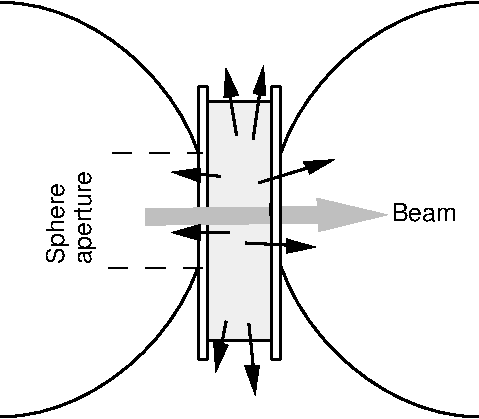
\includegraphics[scale=0.7]{lightloss.pdf}
\end{center}
\caption{Light losses via the sides of the sample holder.  The dashed lines
indicate the diameter of the hole in the integrating sphere.}  
\label{lightloss}
\end{figure}

\noindent
As light is scattered by the sample some may leave the holder
laterally (Figure~\ref{lightloss}).  The amount of light lost will
depend on the thickness $\delta$ of the sample, the diameter of sphere $d$,
the diameter of the sample port $d_s$, and the diameter of the beam $d_b$.

Reflectance and transmittance measurements with a double integrating sphere set-up
were used to find the total collected light for non-absorbing samples with
various physical thicknesses $\delta$, scattering coefficients $\mu_s$, and optical
thicknesses $\mu_s \delta$.  All experiments were done with a 1\,mm  HeNe laser
and various concentrations of Intralipid-10\% to create sample optical
thicknesses that varied from zero to about 55. 

\subsection*{Theory}

The straightforward way of figuring out the total light collected would be
to add the normalized outputs from the reflectance, diffuse transmittance,
and unscattered detectors.  The problem is a simple normalization process
ignores light losses caused by (1) the absorption 
by the sphere walls and (2) light exiting out ports is ignored.
These effects should
be taken into account when using the formulas for a double integrating sphere
apparatus.  This is what Niek did, but he used the formula for a single
integrating sphere to correct his numbers.  He also used a slightly
incorrect form of this equation and therefore his results will be
slightly off (I would guess nor more than 5\%).  Rather than repeat
an incorrect derivation, I'll just skip to the results.

The total light collected was measured for different combinations of the 
sample port size, different sample thicknesses, and different Intralipid
concentrations. The results of these experiments are shown in Figure~\ref{graph}.

\begin{figure}[b!]
\centering
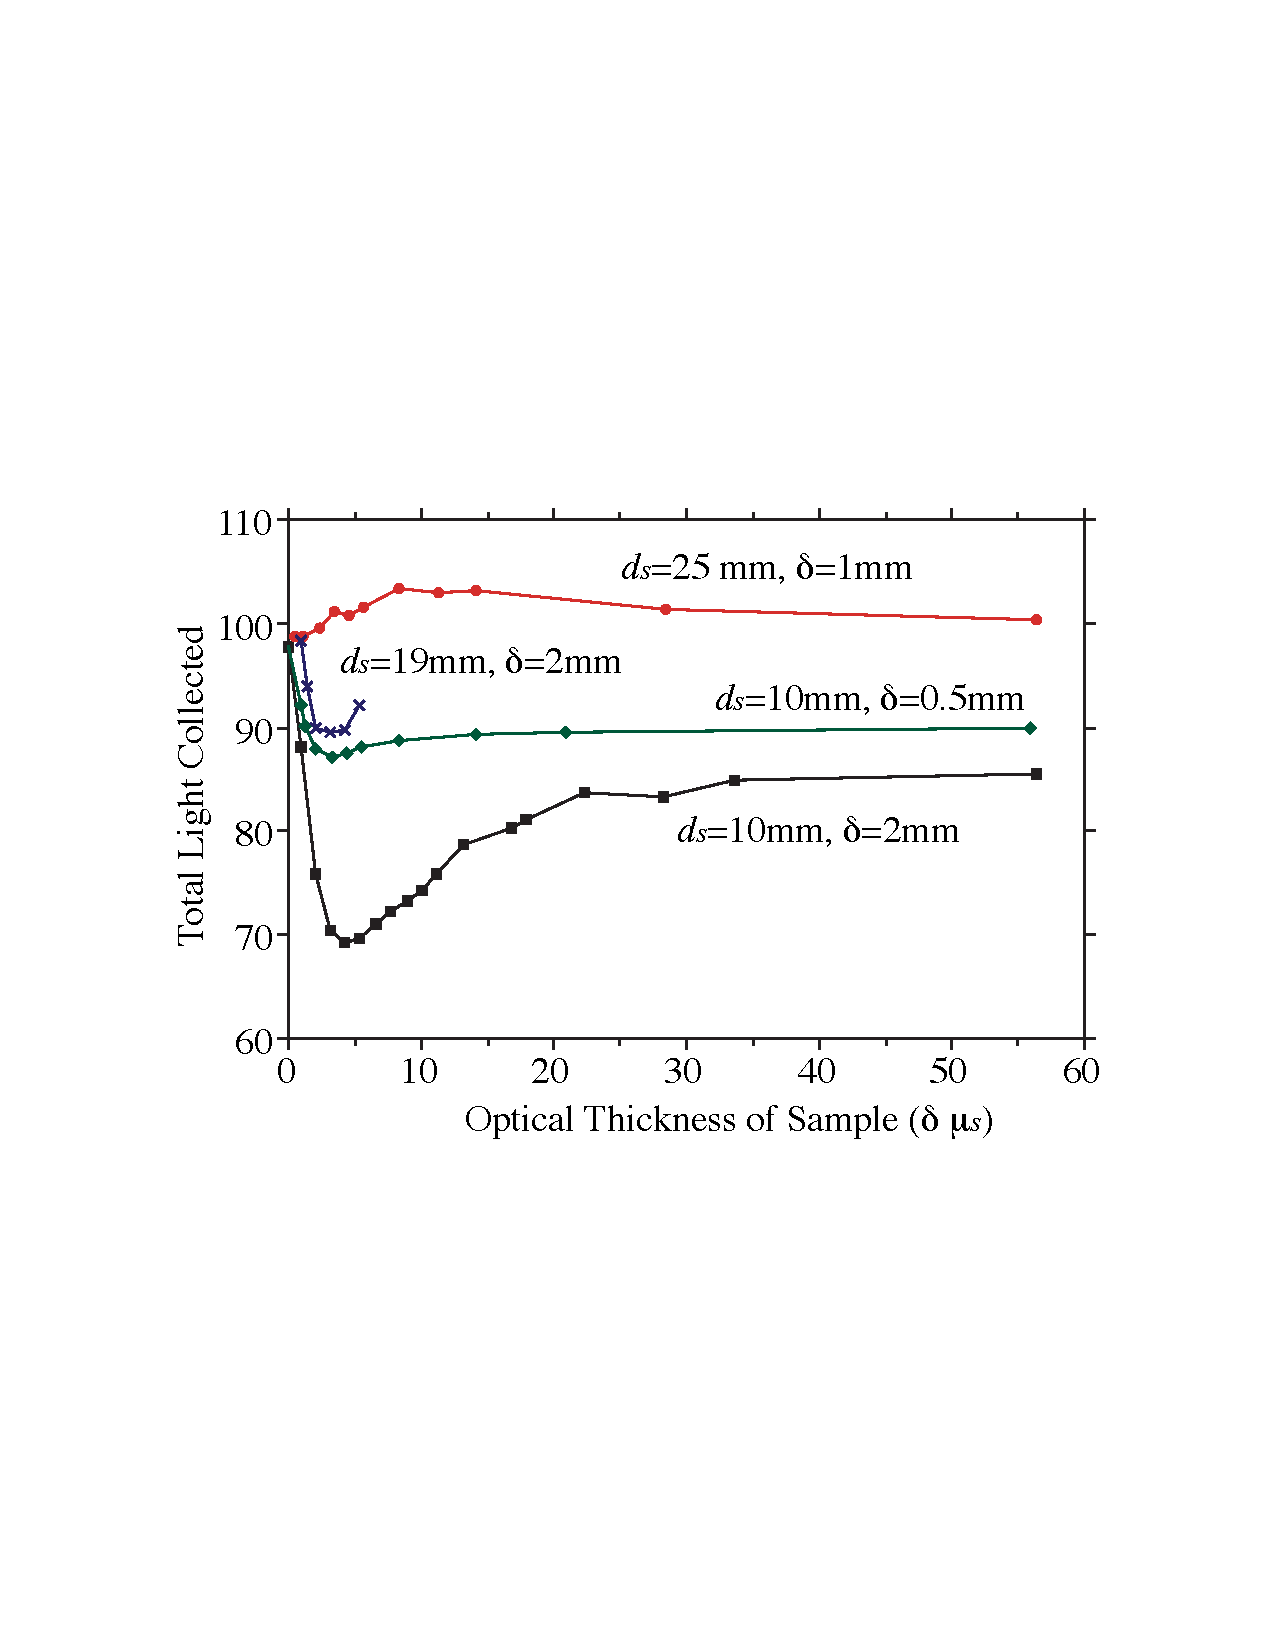
\includegraphics[scale=0.600]{niek_graph.pdf}
\caption{The total collected light versus the optical thickness of the
sample.  Here $\delta$ is the physical thickness of the sample and $d_s$
is the diameter of the sample of the integrating sphere.
The beam diameter was 1\,mm.}
\label{graph}
\end{figure}

\subsection*{Discussion}
The total light collected has roughly the same dependence on the optical
thickness for the three smaller port configurations (Figure~\ref{graph}).  
\begin{enumerate}
    \item 
    When the optical thickness is zero, then there is no scattering and no light is
    lost.  (The total amount of light does not equal 100\% because the specular
    reflectance from the sample was not collected.)

    \item
    As the optical thickness increases, more and more light is scattered.  More
    and more light leave out the edges of the sample until a maximum loss is
    reached.

    \item 
    As the optical thickness increases, so does the optical distance in
    the radial direction.  The radial optical thickness eventually increases 
    to the point that the number of scattering events encountered by photons 
    is so large that they travel only a short distance laterally and
    can no longer escape out the edges.

    \item 
    Eventually the radial optical distance becomes so large that no light escapes
    laterally and the total collected light increases asymptotically to
    a fixed value.  
\end{enumerate}

Consider the curves for a sphere aperture of $d_s=10\,$mm. The maximum discrepancy
occurs for an optical thickness of about four.  When the sample thickness is 2~mm, the total
collected light is always less than when the sample thickness is 0.5~mm.  The
relative radial path lengths are nearly a factor of four greater in the 2~mm 
case, and photons will encounter four times more scattering events before they
might be lost.  
When the sphere aperture is doubled in size $d_s=19\,$mm, then the total light
collected is increased for all optical thicknesses.  

Summarizing, it appears that: 
\begin{itemize}
\item
the overall collection efficiency is determined primarily by ratio of the
radial optical distance to the sample optical thickness,
\item
the limiting value of for the total light collected as the optical thickness
becomes large is primarily determined by the size of the hole in
the sphere.
\end{itemize}
The second point bears closer examination.  In short, the argument is
because the radial optical distance is always larger than
optical depth and therefore as the optical depth becomes large it may be expected
that no light can escape via the sides of the sample holder. 

However, \textit{light does escape} and one mechanism%
\footnote{A second mechanism might be caused by  the diffuse light in the integrating sphere.  Unlike the
relatively small incident beam, all the light in the integrating sphere
is diffuse and uniformly impinges on the entire exposed sample surface.
The diffuse light that hits near the edge of the port has a roughly
50\% chance of being lost.  If this lossy rim area is assumed to be 
roughly one mean free path wide, then the area is given by
$$
\mbox{lossy rim area} = {\pi d_s \over \mu_s'}
$$
The loss will be relative to the total sample area $\pi d_s^2/4$, and
consequently we would expect the light losses due to this effect to 
drop as
$$
{ \pi d_s / \mu_s' \over \pi d_s^2/4} = {4\over \mu_s d_s} = {1\over \delta \mu_s} {4 \delta \over d_s}
$$
This means that the losses should continue to decrease with increasing
optical thicknesses.  This was not observed.}
by which this can happen is
via the the glass slides of the holder, as in Figure~\ref{glass-slide}.  The circle on the top represents light incident at
all angles on a point on the liquid/glass boundary.  The light that
passes this boundary makes angles of at most 59.7$^\circ$ with the
normal of the slide (represented by the cone inside the glass slide). 
At the glass-air boundary, light incident at angles larger than the
critical angle $\theta_c=40.49^\circ$ will be reflected totally and 
otherwise partially.  Also at the glass-liquid boundary light will be
reflected.  If light has been reflected inside the glass slide, a
couple of times it will have travelled some distance in the radial
direction.  For small test apertures the possibility arises that light
is conducted sideways and escapes.  

\begin{figure}[tp]
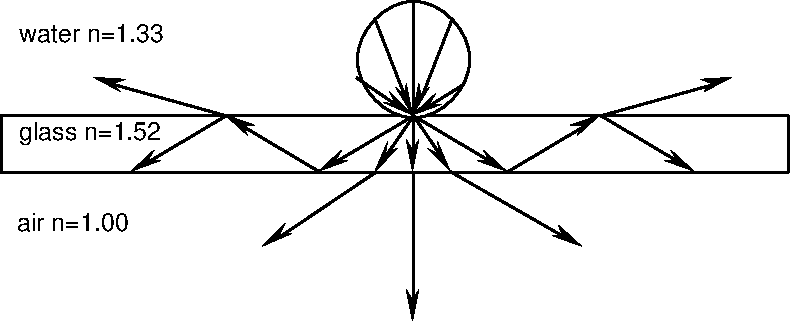
\includegraphics[scale=0.945]{glass-slide.pdf}
\caption{A glass slide with light incident from all possible angles from
the water side.  Since there is no critical angle for the water-air transition
most light will not be reflected by this boundary.  However, total internal
reflectance will occur in the glass slide for all light incident at angles 
greater than 40.5$^\circ$.  This corresponds to angles in the water of greater
than 48.8$^\circ$.  Thus any light incident from the water at angles larger
than this stand a chance of ``walking'' down the inside of the glass slide.}
\label{glass-slide}
\end{figure}


\begin{table}[hbtp]
\centering
\begin{tabular}{lccc}
              &spot radius  &$R=5\,$mm  &$R=12.5\,$mm \\
without glass &$5 \pm1\,$mm &94.3\%			  &94.3\%		 \\
with glass				&$12\pm2\,$mm &83.5\%			  &90.7\%		 \\
\end{tabular}
\caption{The fraction of light collected using a perspex plate with
and without a glass slide in front.  The spot radius is the size of
the glow ball on the perspex.  Both experiments used the same beam
diameter of 1$\,$mm .}
\label{perspex}
\end{table}

This possibility is tested with the following experiment.  A thick piece of
white perspex, strongly scattering and weakly absorbing, is placed in front of
the test aperture of a single sphere set up and percentage of light reflected
is measured.  This measurement is repeated, this time however with a glass
slide against the perspex (`glued' together with a very thin layer of water in
order to minimize  specular reflectance).  The experiment is done for two
different sample port diameters.  The percentage
light that is reflected, is shown in table \ref{perspex}.

The values with and without glass slides cannot and should not be directly compared.%
\footnote{More light will be transmitted through the sample without glass
slides because there are fewer boundaries that can lead to reflected light.}
However, the results for different sample apertures are comparable and
more light is lost when a glass slide is present.  The  glass slide `conducts'
light to the sides of the sample holder.  

This is substantiated by another simple experiment that consists of measuring
the diameter of the glow ball of scattered light in the perspex plate.  When a
glass slide is present the glow ball is more than twice the diameter measured
with the perspex alone (table \ref{perspex}).  A similar effect
also appears when Intralipid is used instead of the perspex plate.  Thus more
light can be recovered by using a larger sample aperture.  This effect is
present in Figure~\ref{lightloss}, where the largest sphere aperture gathered
the most light. However, for this combination the total percentage of collected
light exceeds 100\% .  This of course is physically
impossible, but it has to be taken into account that an approximation is used
to determine the percentage of reflected and diffusely transmitted light. 
Still, this approximation is used in all four combinations and therefore a
relation to one remains useful.


\clearpage
\section*{Appendix 5: Beckman UV 5270 Spectrophotometer}
\addcontentsline{toc}{section}{Appendix 5: Beckman UV 5270 Spectrophotometer}

\subsection*{Introduction}
This memo\footnote{Vasan Venugopalan
at Wellman helped revise this subsection.  So he shares the blame and the glory.}
 is intended to describe how reflectance and transmittance experiments might be 
made with the Beckman UV 5270.   Particular attention is paid to the idiosyncrasies and
limitations of the Beckman.

First things first.  The wavelength is not what it might seem and
it should be understood that the number displayed by the Beckman is
not the number recorded by the PC attached to the Beckman.  For simplicity
we \footnote{Steve Jacques and I spent a week taking data with the 
Beckman back in 1986.  Steve found the A/D converter and I hacked a BASIC
program together that week just to get data.  This is the pretty much the
system that you have now.} choose not to use the digital signal generated by the Beckman, but
rather just took the analog signal out of the back and ran it through
an A/D board.  The output from the A/D board is recorded by the computer.

The measurement need to be divided into four wavelength regions. The UV (250--400~nm),
the visible (400--800~nm), the near-infrared (800--1300~nm), and the less-near-infrared
(1300--2500~nm).  Each will be discussed in turn and skin will be assumed as the
sample. However, before we do this some remarks which are applicable regardless of
wavelength should be mentioned.

\subsection*{General}

\begin{itemize}

\item
The Beckman should be turned on into the warm-up mode and left there for about 10--15
minutes before turning it on completely. The tungsten lamp is used exclusively except
in the UV when the deuterium lamp is needed for extra photo ummph.

\item
For reflectance measurements, the skin sample is placed against a quartz or glass plate
and water was used to match the refractive index of the skin with this plate. Oil was
not used\footnote{Why the worry about oil and water, well if you are interested in
hydration effects then it could be an issue.  Really, I only considered oil because
it has been used on psoriatic lesions to reduce backscattering from the flakey 
outer layers}. Before performing all measurements a 0\% and 99\% reflectance scan must be done. Also
when doing this scan the 0\% and 100\% knobs must be adjusted so that the Beckman never
reads below 0\% or above 100\% for either of these scans over the whole wavelength
region.  Note that the Spectralon reflectance standards should never be put in contact
with oil as it renders them defective (they absorb oil, but are hydrophobic). 
When doing the reference scans no matching fluid
or glass/quartz plate is used.

\item
When performing the transmittance measurements, the sample is placed between two glass or
quartz or glass plates. This sample is placed in front of the sample beam which enters
the sphere. In this case a BaSO$_4$ plate is placed in both the sample and reference
ports. The 0\% and 100\% transmittance measurements are performed by placing either an opaque
or no sample in the path of the beam. When doing these scans the 0\% and 100\% knobs
must be adjusted so that the Beckman never reads below 0\% or above 100\% for either of
these scans over the whole wavelength region. For the tissue samples, water must also be
included to keep the tissue sample hydrated. However when testing epidermis and dermis
make sure that the amount of water added does not artificially increase the thickness
of the sample. Of course for the transmittance measurements the thickness of the sample
must be measured. This is done by measuring the thickness of the quartz/glass plates
used with and without the sample inserted in between.  You need to make several 
measurements in different places because most samples are not very uniform in thickness.

\item
These reference scans should be performed three additional times (e.g., once just before
lunch, once after lunch and definitely once just before shutting the machine down for the
day.) It is also advisable to scan the 10\% or 20\% standards at this time if they are
to be used for the days measurements. The times when this is necessary will become
clearer as you read the rest of this memo.


\end{itemize}

\subsection*{The Ultraviolet}
There are a few problems associated with this region.  

\begin{itemize}

\item
First, the Beckman illuminates with only a single wavelength and detects all light
falling on the detector in the integrating sphere.  This means that if light is
absorbed and the generates fluorescence, much more light will be detected for that
wavelength than should be.  This was pointed out by Rox, in his (in)famous skin optics 
paper \cite{anderson81b}. Rox used a solar-blind photomultiplier tube (Hamamatsu R456)
to prevent detecting visible fluorescence. Thus the same photomultiplier should be used
when making the measurements in the wavelength region 250--300~nm. (It should be in one
of the drawers in the Beckman room.) Ideally these measurements should also be made
with some sort of fluorimeter with the excitation and emission monochromators scanning
at the identical speed and wavelength.

\item
The reflected and transmitted light can be very small (especially for darker skin
types).  The measurements are correspondingly noisy.  We used a 20\% reflectance
plate as the reference target and adjust the 0\% and 100\% dials on the Beckman to
effectively utilize the full range of the machine. As a result 0--100\% will then
correspond to a reflectance between 0 and 20\%.  This improves the generated signal
significantly.  It might be that the electronics in the Beckman just don't work so
well for very small voltages.

\item
Because glass transmits poorly in this region, quartz plates must be used as the
window against which the sample is placed for the reflectance measurement.

\item
Probably most troubling is that in the ultraviolet region the amount of light
falling on the detector is necessarily small.  The Beckman opens and closes the
slits on the monochromator to ensure that the signal stays reasonably constant.
This ensures good signal.  Unfortunately, it also increases the bandpass.  Watch
the dial below the wavelength indicator to get some idea of how large the bandpass
is during a typical scan.  You might be surprised.

\item
Of course this is where you need to use the deuterium lamp.
\end{itemize}

\subsection*{The Visible and Near Infrared (400--1300~nm)}

\begin{itemize}
\item
There is quite a lot of light in this region.  The detector begins to fail at around
800~nm\ (or was it 700~nm?).  Anyway the  spectrophotometer must be adjusted for
infra-red operation.  This  means that the machine must be turned off, and the setting
on the sphere accessory (the lever on the back of the spectrophotometer behind the
sphere) switched to IR mono sphere as well as some dinky little switch near the
wavelength indicator.

\item
Once the machine is working in the infrared, you should be aware  that the
wavelengths now change four times as fast as in the visible. The bandpass indicator
is likewise increased in magnitude.

\item
Also once we are in the infrared you must specify the higher wavelength  as the
starting wavelength $\lambda_s$.  The ending wavelength $\lambda_e$ must be 
$$
\lambda_e=\lambda_s-{\lambda_s-\lambda_e\over4}
$$
because the
computer has no idea that the Beckman is operating in the infrared. For
example if you want to scan from 800~nm to 2500~nm, You set the dial to 2500~nm and
specify the starting wavelength as 2500~nm and the ending wavelength as 2075~nm.

\item
The scan speed is automatically increased by a factor of 4 once we switch into the
IR. Thus scan speed should reduced by depressing the 1/4~nm/s switch from the 4/16~nm/s switch to keep the scan speed at 4~nm/s in the IR.

\end{itemize}

\subsection*{The Near Infrared (1300--2500~nm)}

\begin{itemize}
\item
The reflectance of skin is very poor in this region.  The strong
absorption by water in skin is comparable to or exceeds the scattering
coefficient.  Anyway there is not a whole lot of signal.

\item
The solution once again is to replace the reference plate with a 
10 or 20\% Spectralon standard.  The experiments proceed as for the
ultraviolet.  The absorption by glass is still pretty small and
quartz need not be used.

\item
The 0\% reflectance measurements are a problem.  It turns out that the back
of the sphere door reflects significant amounts of light in this wavelength
range.  I remove the door completely and turn off the room lights and 
sneak off during these calibration scans.  All the scans are done in a 
dark room.  

\end{itemize}

\clearpage

\bibliography{iad}
\bibliographystyle{ieeetr}
\end{document}

 
 